% ОБЯЗАТЕЛЬНО ИМЕННО ТАКОЙ documentclass!
% (Основной кегль = 14pt, поэтому необходим extsizes)
% Формат, разумеется, А4
% article потому что стандарт не подразумевает разделов
% Глава = section, Параграф = subsection
% (понятия "глава" и "параграф" из документа, описывающего диплом)
\documentclass[a4paper,article,14pt]{extarticle}

% Подключаем главный пакет со всем необходимым
\usepackage{spbudiploma_tempora}

% Пакеты по желанию (самые распространенные)
% Хитрые мат. символы
\usepackage{euscript}
% Таблицы
\usepackage{longtable}
\usepackage{makecell}
% Картинки (можно вставлять даже pdf)
\usepackage[pdftex]{graphicx}
\usepackage{float}

\usepackage{amsthm,amssymb, amsmath}
\usepackage{textcomp}

% В шаблоне бакалаврской работы содержание рассчитано на короткие названия
% разделов. Для магистерской ВКР с длинными названиями делаем интервалы шире.
\renewcommand{\cftsecpresnum}{}
\renewcommand{\cftsecaftersnum}{.}
\renewcommand{\cftsubsecaftersnum}{.}
\setlength{\cftsecnumwidth}{3em}
\setlength{\cftsubsecindent}{3em}
\setlength{\cftsubsecnumwidth}{4em}
\setlength{\cftsubsubsecindent}{7em}
\setlength{\cftsubsubsecnumwidth}{5em}
\setlength{\cftbeforesecskip}{7pt}
\setlength{\cftbeforesubsecskip}{3pt}
\setlength{\cftbeforesubsubsecskip}{2pt}
\renewcommand{\cftsecfont}{\normalfont}
\renewcommand{\cftsecpagefont}{\normalfont}
\makeatletter
\renewcommand*{\l@section}[2]{%
  \ifnum \c@tocdepth >\z@
    \addpenalty{\@secpenalty}%
    \addvspace{0.5em}%
    \setlength\@tempdima{2.8em}%
    \begingroup
      \parindent \z@
      \rightskip \@pnumwidth
      \parfillskip -\@pnumwidth
      \leavevmode
      \advance\leftskip\@tempdima
      \hskip -\leftskip
      #1\nobreak\cftsecleader\nobreak
      \hb@xt@\@pnumwidth{\hfil #2}\par
    \endgroup
  \fi}
\makeatother

\begin{document}

% Титульник в файле titlepage_example.tex
\input{titlepage_example.tex}



% Содержание
\setcounter{tocdepth}{3}
\tableofcontents
\pagebreak

\specialsection{Введение}

Машинный перевод является одной из наиболее активно развивающихся областей обработки естественного языка. Если первоначально задача сводилась преимущественно к переводу фрагментов текста, то сейчас всё большую роль играет перевод видеоконтента: лекций, интервью, фильмов, образовательных материалов, видеозаписей рабочих встреч и коротких пользовательских роликов. В такой постановке входными данными является не текст, а видео с речевой дорожкой. Следовательно, система должна не только выполнить перевод, но и извлечь аудио, распознать речь, сохранить временную структуру фраз и сформировать результат в удобном для пользователя виде.

Отдельную сложность представляет поддержка большого числа языков. Для многих языковых пар отсутствуют достаточные для обучения размеченные корпусы текста, поэтому обучение отдельной модели для каждого направления оказывается неэффективным. В таких условиях естественным образом возникает задача zero-shot translation: перевод между языками, для которых модель не обучалась на корпусе параллельных данных~\cite{Google}.

Настоящая работа развивает результаты предыдущих исследований~\cite{Devrishev2023} в прикладном направлении. Если ранее основной интерес представляло качество текстового zero-shot перевода, то в данной работе рассматривается полный процесс перевода видеоконтента. Центральным результатом является программная платформа, объединяющая извлечение аудио, распознавание речи, перевод, синтез речи и сборку видео с заменённой аудиодорожкой.

Практическая важность такой системы определяется тем, что видеоконтент становится одним из основных способов передачи информации. Качественный перевод видео вручную требует времени, участия переводчиков, дикторов и специалистов по монтажу. Для образовательных материалов и научно-технических докладов это особенно существенно: задержка между появлением исходного материала и его переводом снижает доступность знаний для аудитории, не владеющей исходным языком. Автоматизация процесса позволяет быстрее получать перевод, который затем может использоваться как конечный результат или как основа для ручной доработки.

Разрабатываемая платформа должна поддерживать выбор из нескольких моделей перевода, рекомендации по метрикам качества, отслеживание задач и администрирование сведений о моделях; перечень требований приведён в постановке задачи.

\newpage
\specialsection{Постановка задачи}

Целью работы является разработка системы перевода видеоконтента с использованием zero-shot translation.

В данной работе рассматривается задача автоматического перевода видеоконтента с одного языка на другой. На вход системе подается видеофайл, содержащий речевую дорожку на исходном языке. На выходе необходимо получить видео с речевой дорожкой на целевом языке.

К системе предъявляются следующие функциональные требования:
\begin{enumerate}
  \item Выбор одной из нескольких доступных моделей перевода.
  \item Рекомендация модели перевода для выбранной языковой пары на основании метрик качества перевода; пользователь может принять рекомендацию или выбрать модель вручную.
  \item Отображение статуса и прогресса выполнения задачи до завершения обработки или возникновения ошибки.
  \item Сохранение переведённого видео как результата обработки; в дальнейшем --- возможность скачивания готового файла.
  \item Административный интерфейс для управления сведениями о моделях, поддерживаемых языковых парах и метриках качества перевода.
\end{enumerate}

Помимо этого, к системе предъявляются следующие нефункциональные требования:
\begin{enumerate}
  \item Простое подключение новых моделей распознавания речи, перевода и синтеза речи без перестройки остальной системы.
  \item Устойчивость к сбоям: корректная обработка ошибок, повторный запуск прерванных задач.
  \item Наблюдаемость: журналирование этапов обработки и возможность отслеживать состояние задач и воркеров при эксплуатации.
  \item Сохранение промежуточных артефактов обработки для отладки и диагностики сбоев.
\end{enumerate}

Результатом работы будет являться система автоматического перевода видеоконтента: пользователь передаёт видео с речью на исходном языке и получает видео с озвучкой на целевом. Система гибкая --- допускает подключение нескольких моделей распознавания речи, перевода и синтеза речи и позволяет выбирать модель под конкретную задачу. Для пользователя она удобна: доступны рекомендация модели по метрикам качества для выбранной языковой пары, отслеживание хода обработки и сохранение готового результата. Для сопровождения и развития предусмотрены администрирование сведений о моделях и языковых парах, наблюдаемость при эксплуатации, устойчивость к сбоям и сохранение промежуточных данных для диагностики.

\newpage
\specialsection{Обзор литературы}

Основой данной работы является концепция zero-shot translation. Одной из ключевых работ в этой области является статья исследователей Google, в которой была представлена многоязычная нейронная система машинного перевода~\cite{Google}. Авторы показали, что одна модель имеет возможность осуществлять перевод для многих пар языков, если на вход добавлять специальный токен целевого языка. Наиболее важным результатом этой работы стало наблюдение, что модель способна выполнять перевод и для тех языковых направлений, которые не были явно представлены в обучающих данных.

Архитектурной основой большинства современных систем машинного перевода является Transformer~\cite{Attention}. В отличие от рекуррентных моделей, Transformer использует механизм self-attention, позволяющий учитывать связи между токенами последовательности независимо от расстояния между ними. Для задач перевода это особенно важно, поскольку соответствующие друг другу слова и конструкции в разных языках могут находиться в разных позициях предложения. В настоящей работе Transformer рассматривается как общий фундамент современных моделей: NLLB, SeamlessM4T, Whisper и систем синтеза речи (text-to-speech, TTS).

Важным источником данных для машинного перевода являются открытые параллельные корпусы. Проект OPUS был создан как коллекция параллельных данных, извлеченных из открытых источников~\cite{opus_1}. Для данной работы особенно важен корпус OpenSubtitles --- параллельные реплики к фильмам и сериалам~\cite{opus_2}. Такие данные близки к предметной области перевода видео: предложения обычно короче, часто содержат разговорную речь, а качество перевода связано не только с грамматической корректностью, но и с естественностью фраз.

Для оценки качества машинного перевода традиционно используются автоматические метрики. BLEU сравнивает перевод-кандидат с эталонным переводом на уровне n-грамм~\cite{bleu}. Метрика удобна тем, что позволяет быстро сравнивать несколько моделей на одном тестовом наборе, однако она не всегда отражает смысловую близость перевода, особенно если допустимо несколько корректных вариантов. NIST развивает идею BLEU, но придает больший вес более информативным n-граммам~\cite{nist}.

Для распознавания речи существенное значение имеет модель \foreignlanguage{english}{Whisper} \cite{Whisper}. Она основана на архитектуре encoder-decoder Transformer и обучалась на большом объеме слабора размеченных многоязычных аудиоданных. В контексте перевода видео Whisper важна не только как модель автоматического распознавания речи (automatic speech recognition, ASR), но и как практический инструмент сегментации речи с временными метками. Это позволяет согласовывать этапы перевода и синтеза речи с исходным видео.

Отдельное направление исследований связано с end-to-end переводом речи. Модель ZeroSwot ориентирована на zero-shot speech translation и использует речевой энкодер, связанный с пространством текстовой модели машинного перевода~\cite{ZeroSwot}. Идея данного подхода состоит в том, чтобы использовать сильную многоязычную модель перевода, но расширить ее на речевой вход. Для настоящей работы ZeroSwot может быть подключён как один из переводчиков в модульной схеме перевода видео.

SeamlessM4T является более универсальной системой, поддерживающей перевод речи и текста для большого числа языков~\cite{SeamlessM4T}. В отличие от каскадных решений, где распознавание речи, перевод и синтез речи являются независимыми компонентами, SeamlessM4T строится как мультимодальная система, объединяющая несколько направлений: speech-to-text, speech-to-speech, text-to-text и text-to-speech. Для данной работы это особенно важно, поскольку такая модель естественно соответствует задаче перевода видеоконтента.

Для синтеза речи в целевом языке существенны модели multilingual text-to-speech. XTTS относится к классу многоязычных zero-shot TTS-моделей и позволяет синтезировать речь на разных языках, используя ограниченный объем информации о голосе~\cite{XTTS}. В рамках данной работы TTS-компонент рассматривается как заменяемый модуль: архитектура платформы должна позволять собирать озвученную версию видео с заменённой аудиодорожкой.

\newpage
\section{Подходы к решению задачи}

В данной главе рассматриваются подходы, на которые опирается разрабатываемая платформа: многоязычный перевод текста, zero-shot перевод текста, а также перевод видеоконтента. Помимо этого, приводятся отличия предлагаемого решения от распространённых альтернатив.

\subsection{Многоязычный перевод}

Классическая задача машинного перевода предполагает обучение модели для одной языковой пары. Например, если необходимо осуществлять перевод с немецкого на английский, для обучения модели используется корпус параллельных предложений $\textbf{De}\!\rightarrow\!\textbf{En}$, после чего модель применяется именно к данной языково паре. Такой простой подход показывает неплохие результаты при наличии большого числа качественных параллельных данных, но плохо масштабируется на множество языков: при $n$ поддерживаемых языках число потенциальных направлений перевода растёт квадратично, т.к. для каждой пары языков необходимо обучить отдельную модель.

Многоязычный машинный перевод решает эту проблему обучением одной модели для нескольких языковых пар. Часть параметров используется совместно для разных языков, что позволяет переносить знания между направлениями. Например, модель, обученная на корпусах текста $\textbf{De}\!\rightarrow\!\textbf{En}$ и $\textbf{En}\!\rightarrow\!\textbf{Uk}$, может частично использовать общие представления для немецкого, английского и украинского языков. Для управления целевым языком в многоязычных моделях часто добавляют специальный токен: входная последовательность дополняется меткой вида \textbf{<2tgt>}, где \textbf{tgt} обозначает целевой язык. Несмотря на свою простоту, приём широко применяется в современных многоязычных моделях машинного перевода~\cite{Google}.

Zero-shot translation является задачей перевода в условиях, когда для интересующей языковой пары отсутствует прямой параллельный корпус данных. Например, при обучении модели машинного перевода на корпусах $\textbf{De}\!\rightarrow\!\textbf{En}$ и $\textbf{En}\!\rightarrow\!\textbf{Uk}$, задачей zero-shot будет перевод в направлении $\textbf{De}\!\rightarrow\!\textbf{Uk}$, несмотря на отсутствие корпуса данных для этой пары. Главное преимущество --- поддержка большего числа направлений. Для платформы перевода видео это свойство является полезным, поскольку позволяет увеличить количество поддерживаемых языковых пар. Однако недостатком является нестабильность качества: модель может неверно выбрать целевой язык, исказить смысл или перейти к языку-посреднику. Как было показано~\cite{Devrishev2023}, использование лексически близкого языка с дополнительными данными может улучшить качество zero-shot перевода.

\begin{figure}[ht]
\begin{center}
\scalebox{0.2}{
   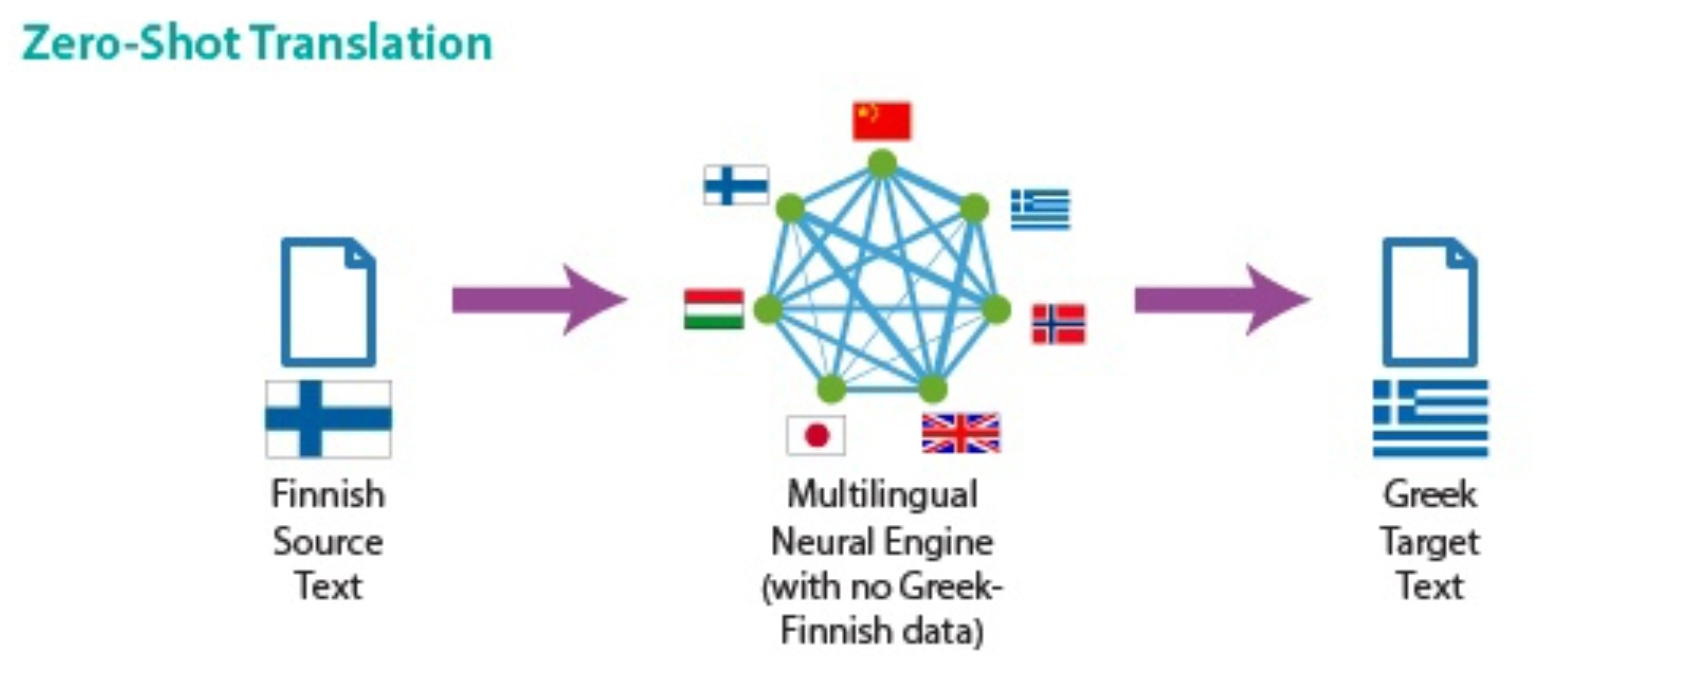
\includegraphics{images/zst.jpeg}
}
\caption{
\label{fig:zst}
     Zero-shot translation.}
\end{center}
\end{figure}

\subsection{Перевод видеоконтента}

Задача перевода видеоконтента отличается от задачи перевода готового текста. Исходная речь разбита на временные сегменты; слишком длинные сегменты усложняют синтез и монтаж, а слишком короткие могут разрушать контекст. В речи встречаются паузы, повторы и незаконченные фразы; перевод и озвучка должны быть согласованы с длительностью исходного видеоряда. При замене аудиодорожки переведённая фраза может не поместиться в исходный временной интервал, поэтому возникает необходимость в изменении темпа речи, пересегментации или допустимой частичной рассинхронизации.

На практике выделяют два семейства решений: каскадный подход и end-to-end подход.

\subsubsection{Каскадный подход}

Каскадный подход предполагает декомпозицию задачи на последовательность этапов: извлечение аудио, распознавание речи, машинный перевод, синтез речи и сборка итогового видео. Каждый этап выполняется отдельным компонентом или моделью, а промежуточные результаты могут быть сохранены, проверены и при необходимости исправлены.

Преимущество такого подхода состоит в управляемости программной системы. Отдельные компоненты можно заменять независимо: например, использовать одну модель для распознавания речи, другую модель для перевода и отдельную модель синтеза речи. Это может быть полезно для платформы, в которой требуется поддерживать несколько моделей машинного перевода и постепенно расширять набор языковых пар.

Основной недостаток каскадного подхода связан с накоплением ошибок. Ошибка распознавания речи передаётся на этап перевода, а затем может быть воспроизведена при синтезе речи. Кроме того, необходимо дополнительно согласовывать сегментацию, длительность фраз и итоговую синхронизацию с видеорядом.

\subsubsection{End-to-end подход}

End-to-end подход предполагает более прямое решение задачи: на вход модели подается аудио дорожка на исходном языке, из которой модель формирует текст или речь на целевом языке, минуя часть промежуточных этапов. Такой подход концептуально ближе к постановке перевода речи, поскольку модель может учитывать акустические признаки, интонацию и паузы исходной записи.

Недостатком end-to-end подхода является меньшая прозрачность результата. Если качество перевода оказывается неудовлетворительным, гораздо сложнее определить, на каком этапе возникла ошибка: при распознавании, переводе или генерации речи. Для прикладной платформы это существенно, поскольку при эксплуатации могут быть важны диагностика, повторный запуск отдельных этапов и возможность анализа промежуточных артефактов.

\subsection{Сравнение с аналогами}

Существующие способы получить переведённое видео можно условно разделить на несколько классов.

\subsubsection{Облачные сервисы автоматической локализации}

Данный подход заключается в использовании внешнего сервиса, который предоставляет готовый конвейер обработки: пользователь загружает видео, выбирает параметры перевода и получает итоговый файл. Основная логика распознавания речи, перевода, синтеза и сборки результата скрыта внутри сервиса.

Недостаток такого подхода состоит в ограниченной управляемости. Пользователь, как правило, не выбирает конкретные модели распознавания и перевода, не видит промежуточные результаты и не может сопоставить несколько переводчиков для одной языковой пары по заранее рассчитанным метрикам качества. Кроме того, зависимость от внешнего сервиса усложняет воспроизводимость экспериментов и контроль над данными.

Разрабатываемая платформа решает эти ограничения за счёт явного управления моделями и задачами обработки. Пользователь может выбрать одну из нескольких подключённых моделей или принять рекомендацию системы, а промежуточные артефакты сохраняются для диагностики и повторного анализа. Такой подход делает процесс более прозрачным и пригодным как для эксплуатации, так и для исследовательского сравнения переводчиков.

\subsubsection{Исследовательские и узкоспециализированные конвейеры обработки}

Данный подход заключается в построении программного конвейера вокруг одной модели, одного набора данных или одного сценария применения. Такие решения часто создаются для проверки гипотезы: например, для оценки конкретного переводчика, обработки одной языковой пары или формирования только одного типа выходного результата.

Недостаток заключается в слабой пригодности к расширению и эксплуатации. Обычно такие конвейеры обработки не имеют единого интерфейса задач, не поддерживают администрирование сведений о моделях и языковых парах, а повторный запуск отдельных этапов требует ручного вмешательства. При добавлении новой модели часто приходится изменять значительную часть кода.

Разрабатываемая платформа устраняет эти ограничения модульной архитектурой. Распознавание речи, перевод и синтез речи представлены как заменяемые компоненты, а новые модели подключаются через единый контракт. Обработка оформляется как управляемая задача со статусом, прогрессом и сохранением промежуточных результатов, что повышает воспроизводимость и упрощает дальнейшее развитие системы.

\subsubsection{Встроенные средства видеоплатформ}

Данный подход предполагает использование функций перевода, встроенных в платформу размещения или просмотра видео. В этом случае перевод является вспомогательной возможностью самой площадки, а пользователь работает в рамках её интерфейса и поддерживаемого набора языков.

Недостаток такого подхода состоит в зависимости от ограничений конкретной площадки. Пользователь не управляет набором моделей, не может подключить собственный переводчик, а качество и доступность языковых направлений определяются внешней системой. Кроме того, такие средства плохо подходят для независимой обработки собственных материалов вне выбранной платформы.

Разрабатываемая система не привязана к конкретному видеохостингу и ориентирована на самостоятельную обработку входных файлов. Она позволяет хранить сведения о поддерживаемых языковых парах, выбирать модель перевода, отслеживать выполнение задачи и сохранять итоговое видео. За счёт этого платформа может использоваться как независимое прикладное решение и как основа для последующей интеграции с разными пользовательскими интерфейсами.

\newpage
\section{Архитектура разрабатываемой системы}

\subsection{Общая схема}

Архитектура системы проектируется исходя из того, что перевод видео является длительной операцией и не должен выполняться внутри пользовательского HTTP-запроса. Пользовательский интерфейс должен быстро реагировать на действия пользователя, а запуск моделей распознавания, перевода и синтеза речи должен происходить отдельно, в управляемом фоновом контуре. Поэтому система разделяется на компоненты, отвечающие за пользовательский сценарий, управление задачами, хранение данных и выполнение ресурсоёмкой обработки.

\begin{figure}[H]
\begin{center}
   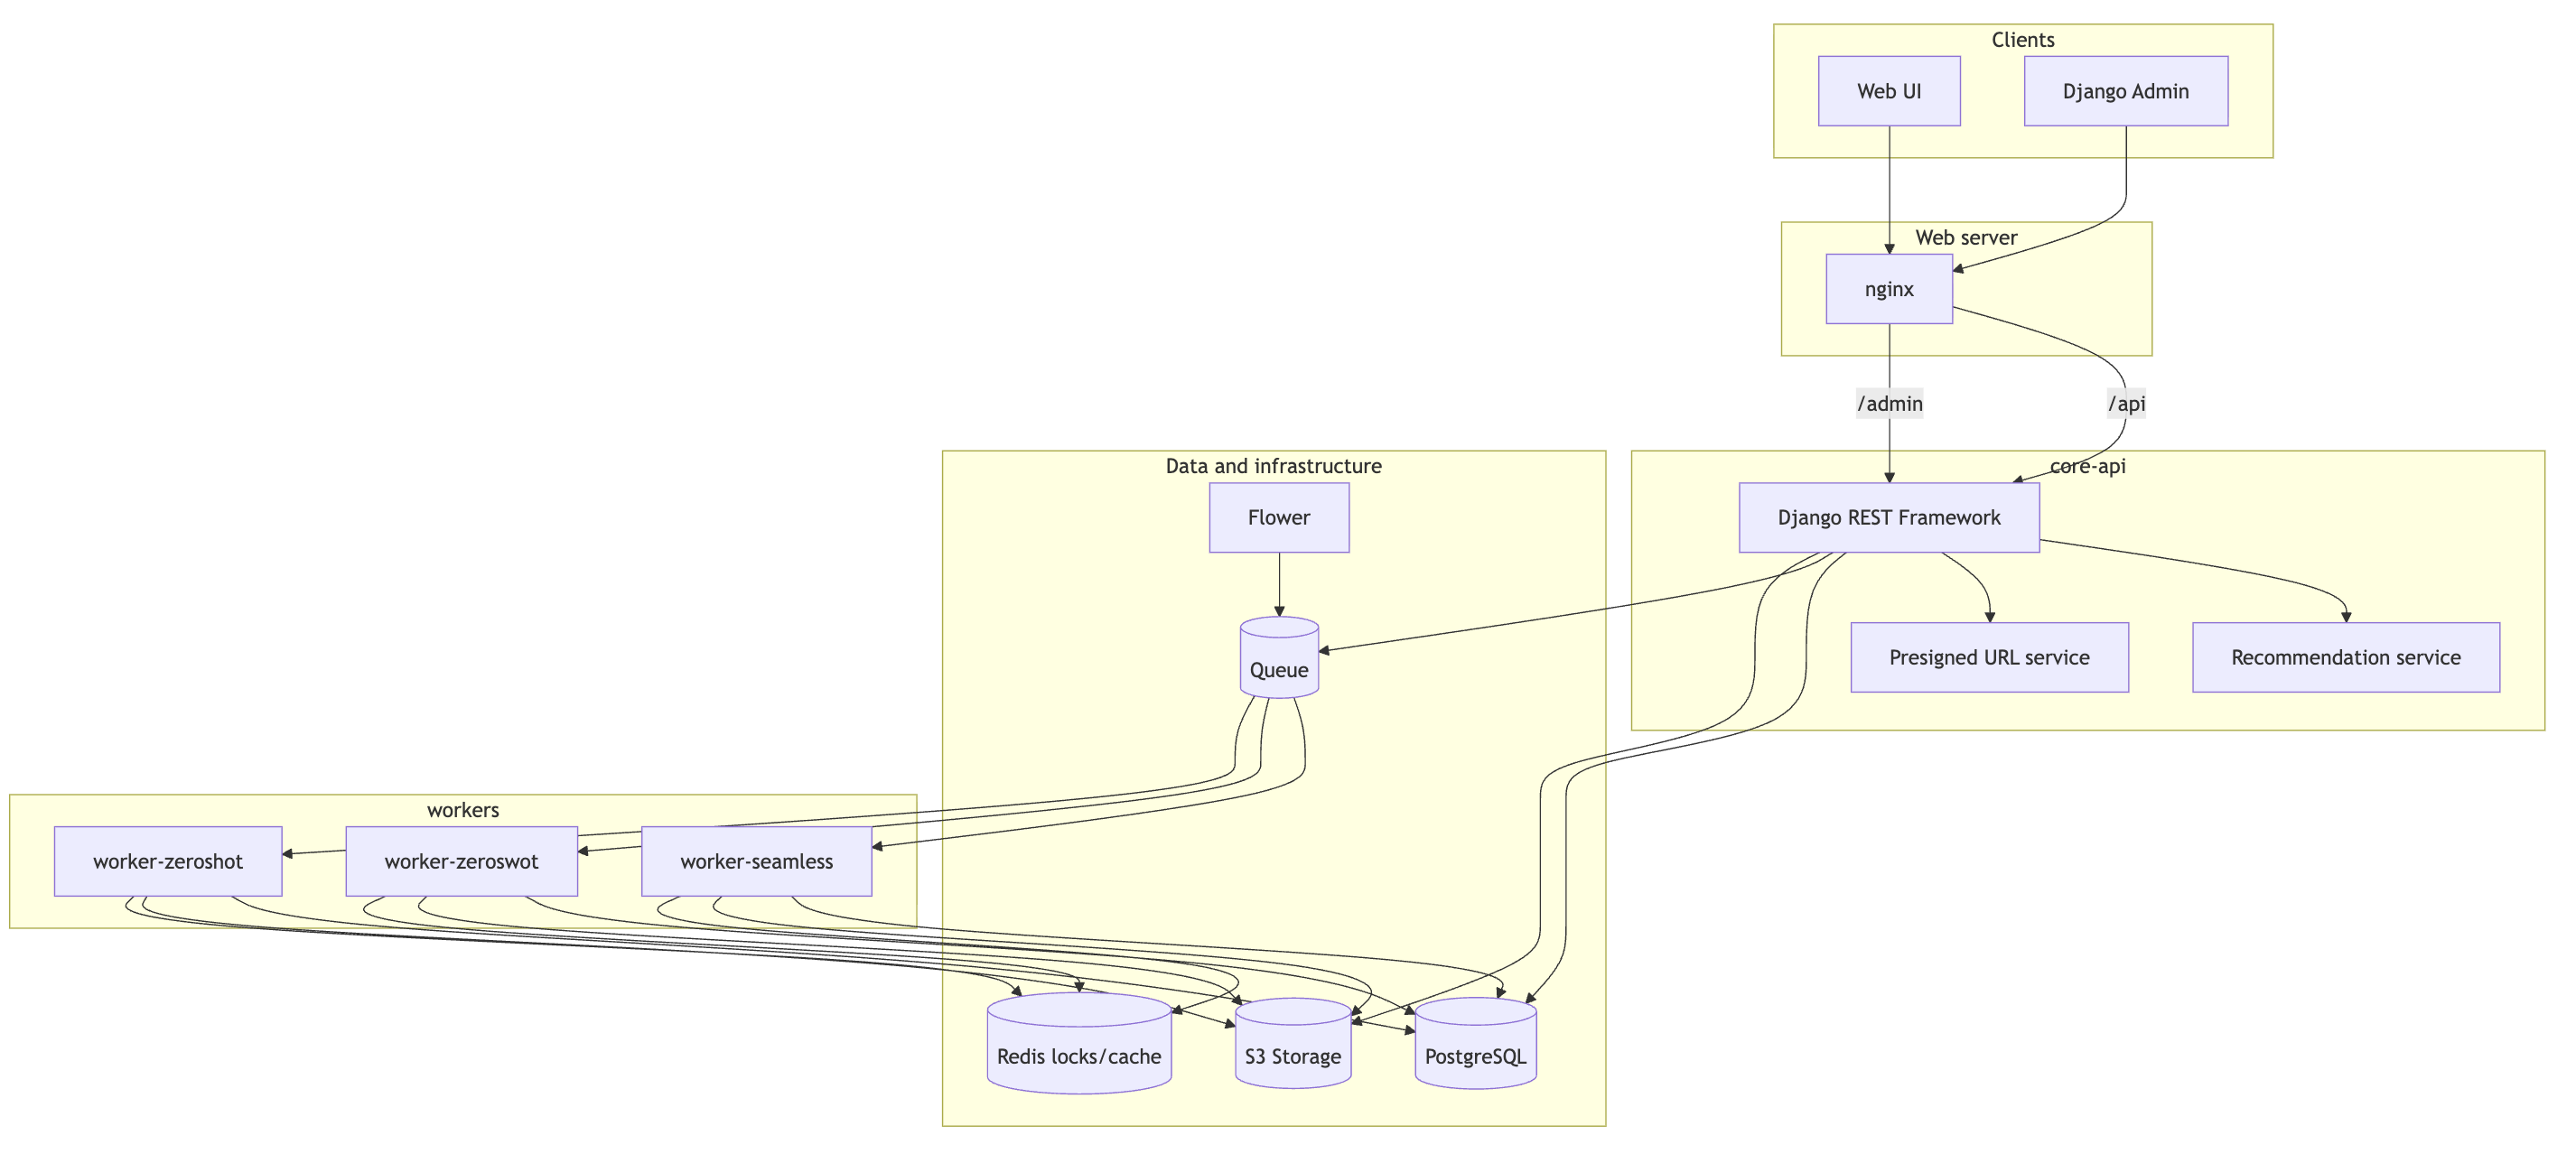
\includegraphics[width=0.95\textwidth]{images/general.png}
\caption{
\label{fig:general-architecture}
     Общая архитектура системы.}
\end{center}
\end{figure}

Центральная идея архитектуры состоит в отделении бэкенда от обработчиков. Бэкенд принимает запросы, проверяет параметры, создаёт задачу и передаёт её в очередь. Обработчик получает задачу асинхронно и выполняет перевод видео независимо от жизненного цикла пользовательского соединения. Благодаря этому пользователь может закрыть страницу или продолжить работу, а состояние задачи сохраняется в базе данных и остаётся доступным для последующего просмотра.

Файлы также не передаются через базу данных. Исходное видео, промежуточные артефакты и итоговый результат хранятся в объектном хранилище, а в базе фиксируются только ключи объектов и метаданные. Такой подход лучше соответствует природе видеоданных: файлы могут быть большими, а база данных должна оставаться хранилищем структурированной информации о задачах, моделях и языковых парах.

На рис.~\ref{fig:general-architecture} показано, что пользователь работает только с фронтендом, а фронтенд обращается к бэкенду. Бэкенд является точкой входа для программного интерфейса: он не содержит логики непосредственно перевода видео, но связывает пользовательский сценарий с базой данных, очередью задач и объектным хранилищем. Система администрирования использует те же данные, но предназначена не для обычного пользователя, а для сопровождения моделей, языковых пар и метрик качества.

Обработчики вынесены в отдельный слой, поскольку именно они запускают тяжёлые модели и работают с видеофайлами. Каждый обработчик может быть настроен под конкретный сценарий перевода: собственную zero-shot схему, ZeroSwot или SeamlessM4T. Такое разделение позволяет обновлять и масштабировать обработчики независимо от фронтенда и бэкенда.

Инфраструктурные компоненты выполняют вспомогательную, но критически важную роль. Очередь связывает бэкенд и обработчики, объектное хранилище служит общим местом для файлов, а система мониторинга позволяет наблюдать за задачами и состоянием обработчиков. В результате архитектура становится не просто набором модулей машинного обучения, а полноценной платформой для длительной асинхронной обработки видео.

Типовой пользовательский сценарий представлен на рис.~\ref{fig:sequence-flow}. Пользователь выбирает языковую пару и модель, загружает видео, после чего бэкенд создаёт задачу и передаёт её обработчику. Пока задача выполняется, фронтенд периодически запрашивает состояние обработки и показывает прогресс.

\begin{figure}[H]
\begin{center}
   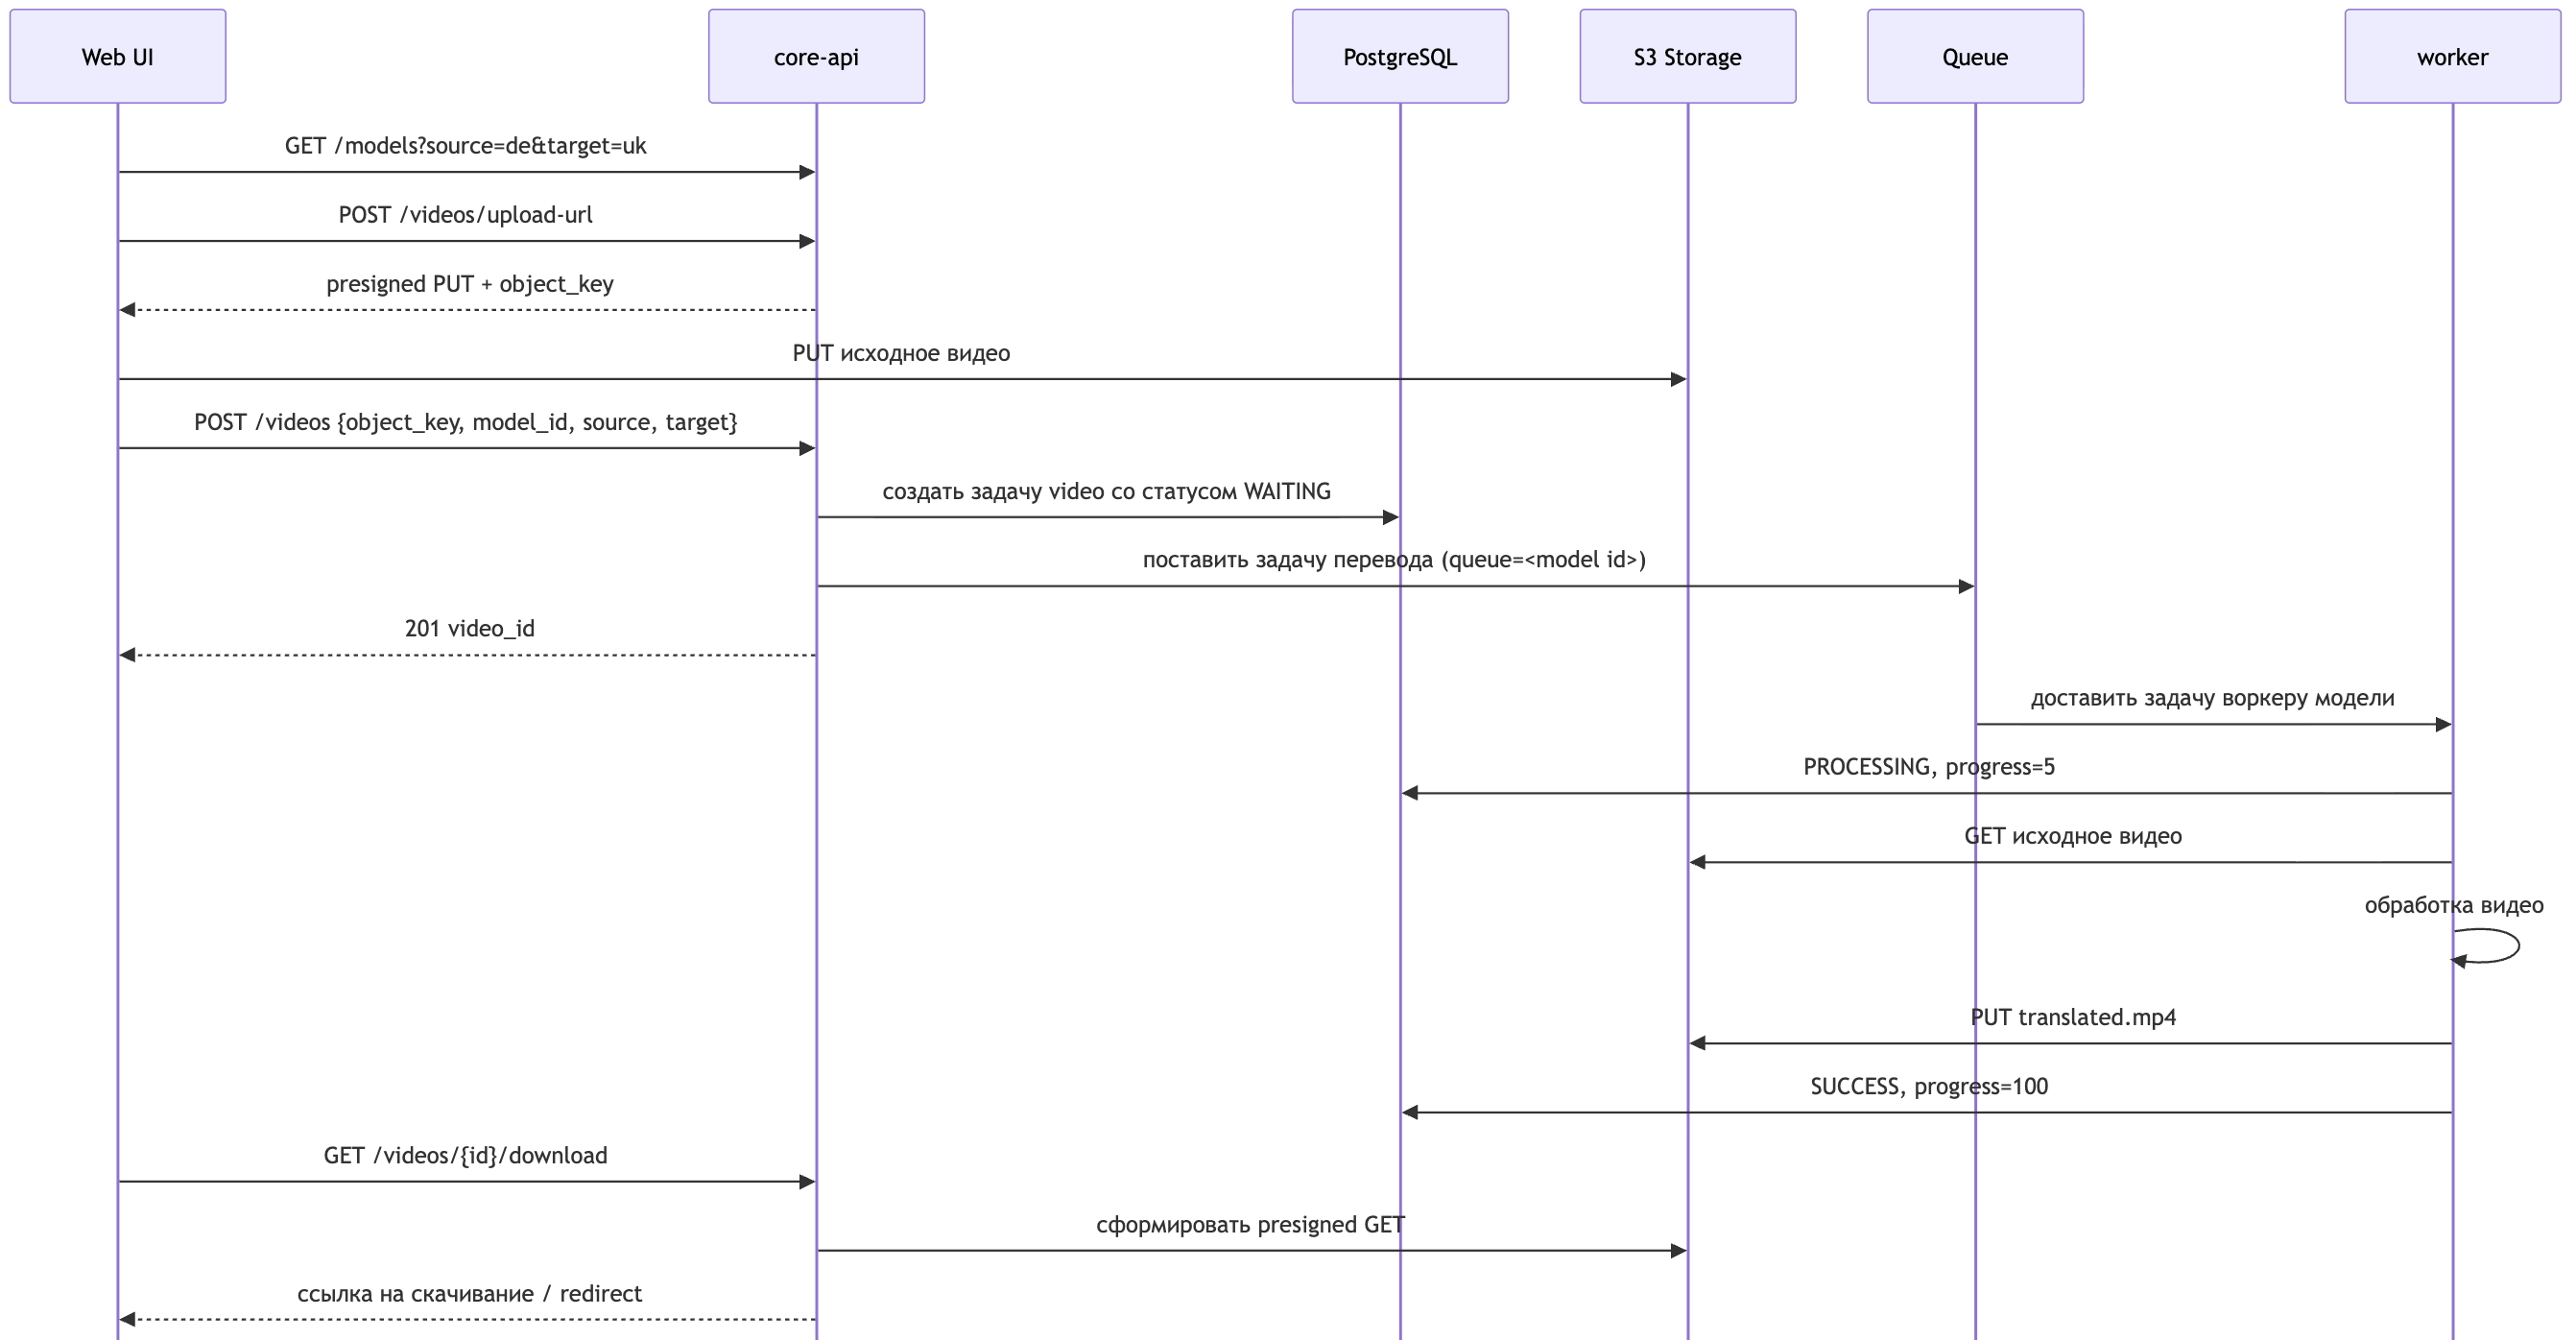
\includegraphics[width=0.95\textwidth]{images/sequence.png}
\caption{
\label{fig:sequence-flow}
     Последовательность обработки пользовательского запроса.}
\end{center}
\end{figure}

\subsection{Отказоустойчивость}

Отказоустойчивость платформы рассматривается как способность системы продолжать работу при выходе из строя одного из её экземпляров или серверов. Например, если один сервер с бэкендом перестаёт отвечать, входящий трафик должен быть перенаправлен на другой экземпляр бэкенда. Для этого бэкенд проектируется как stateless-компонент: он не хранит состояние задачи в памяти процесса, а обращается к общей базе данных и объектному хранилищу.

Отказ отдельного обработчика также не должен приводить к потере всей платформы. Задачи поступают в обработчики через очередь, поэтому при недоступности одного экземпляра другие обработчики могут продолжить получать новые сообщения. Если обработчик завершился аварийно во время выполнения задачи, очередь и механизм повторной доставки позволяют вернуть задачу в обработку после восстановления или передачи другому экземпляру.

Общие компоненты хранения должны размещаться отдельно от вычислительных экземпляров. База данных хранит метаданные задач и не зависит от памяти конкретного бэкенда или обработчика. Объектное хранилище содержит исходные видео, промежуточные артефакты и результаты, поэтому отказ одного сервера приложения не приводит к потере файлов. Для практической эксплуатации такие компоненты должны разворачиваться с резервированием или использовать управляемые сервисы, где репликация и восстановление обеспечиваются на уровне инфраструктуры.

\subsection{Масштабируемость}

Масштабирование системы разделяется на две части: масштабирование пользовательских запросов и масштабирование обработки видео. Фронтенд и бэкенд являются относительно лёгкими компонентами: они обслуживают выбор языков, создание задач, периодический опрос статусов и выдачу ссылок на файлы. Их можно масштабировать горизонтально, увеличивая число экземпляров за обратным прокси-сервером.

Обработчики масштабируются иначе, поскольку именно они используют CPU, память и GPU. Для разных моделей целесообразно иметь отдельные очереди и отдельные группы обработчиков: SeamlessM4T, ZeroSwot и собственная zero-shot схема могут иметь разные зависимости и разное время обработки. Если нагрузка на одну модель растёт, можно увеличить число обработчиков только для соответствующей очереди, не изменяя бэкенд и фронтенд.

Разбиение видео на фрагменты длительностью 5 секунд также помогает масштабированию. Во-первых, прогресс задачи можно считать по числу обработанных фрагментов. Во-вторых, при развитии системы фрагменты могут стать единицей параллельной обработки: разные фрагменты одного видео можно обрабатывать независимо и затем склеивать в итоговую аудиодорожку.

\newpage
\section{Реализация}

\subsection{Фронтенд}

Фронтенд реализует пользовательский сценарий работы с платформой. Пользователь выбирает языковую пару, видит доступные модели перевода, получает рекомендацию, загружает видео и наблюдает за изменением статуса задачи. После завершения обработки интерфейс предоставляет доступ к готовому результату.

\begin{figure}[H]
\begin{center}
   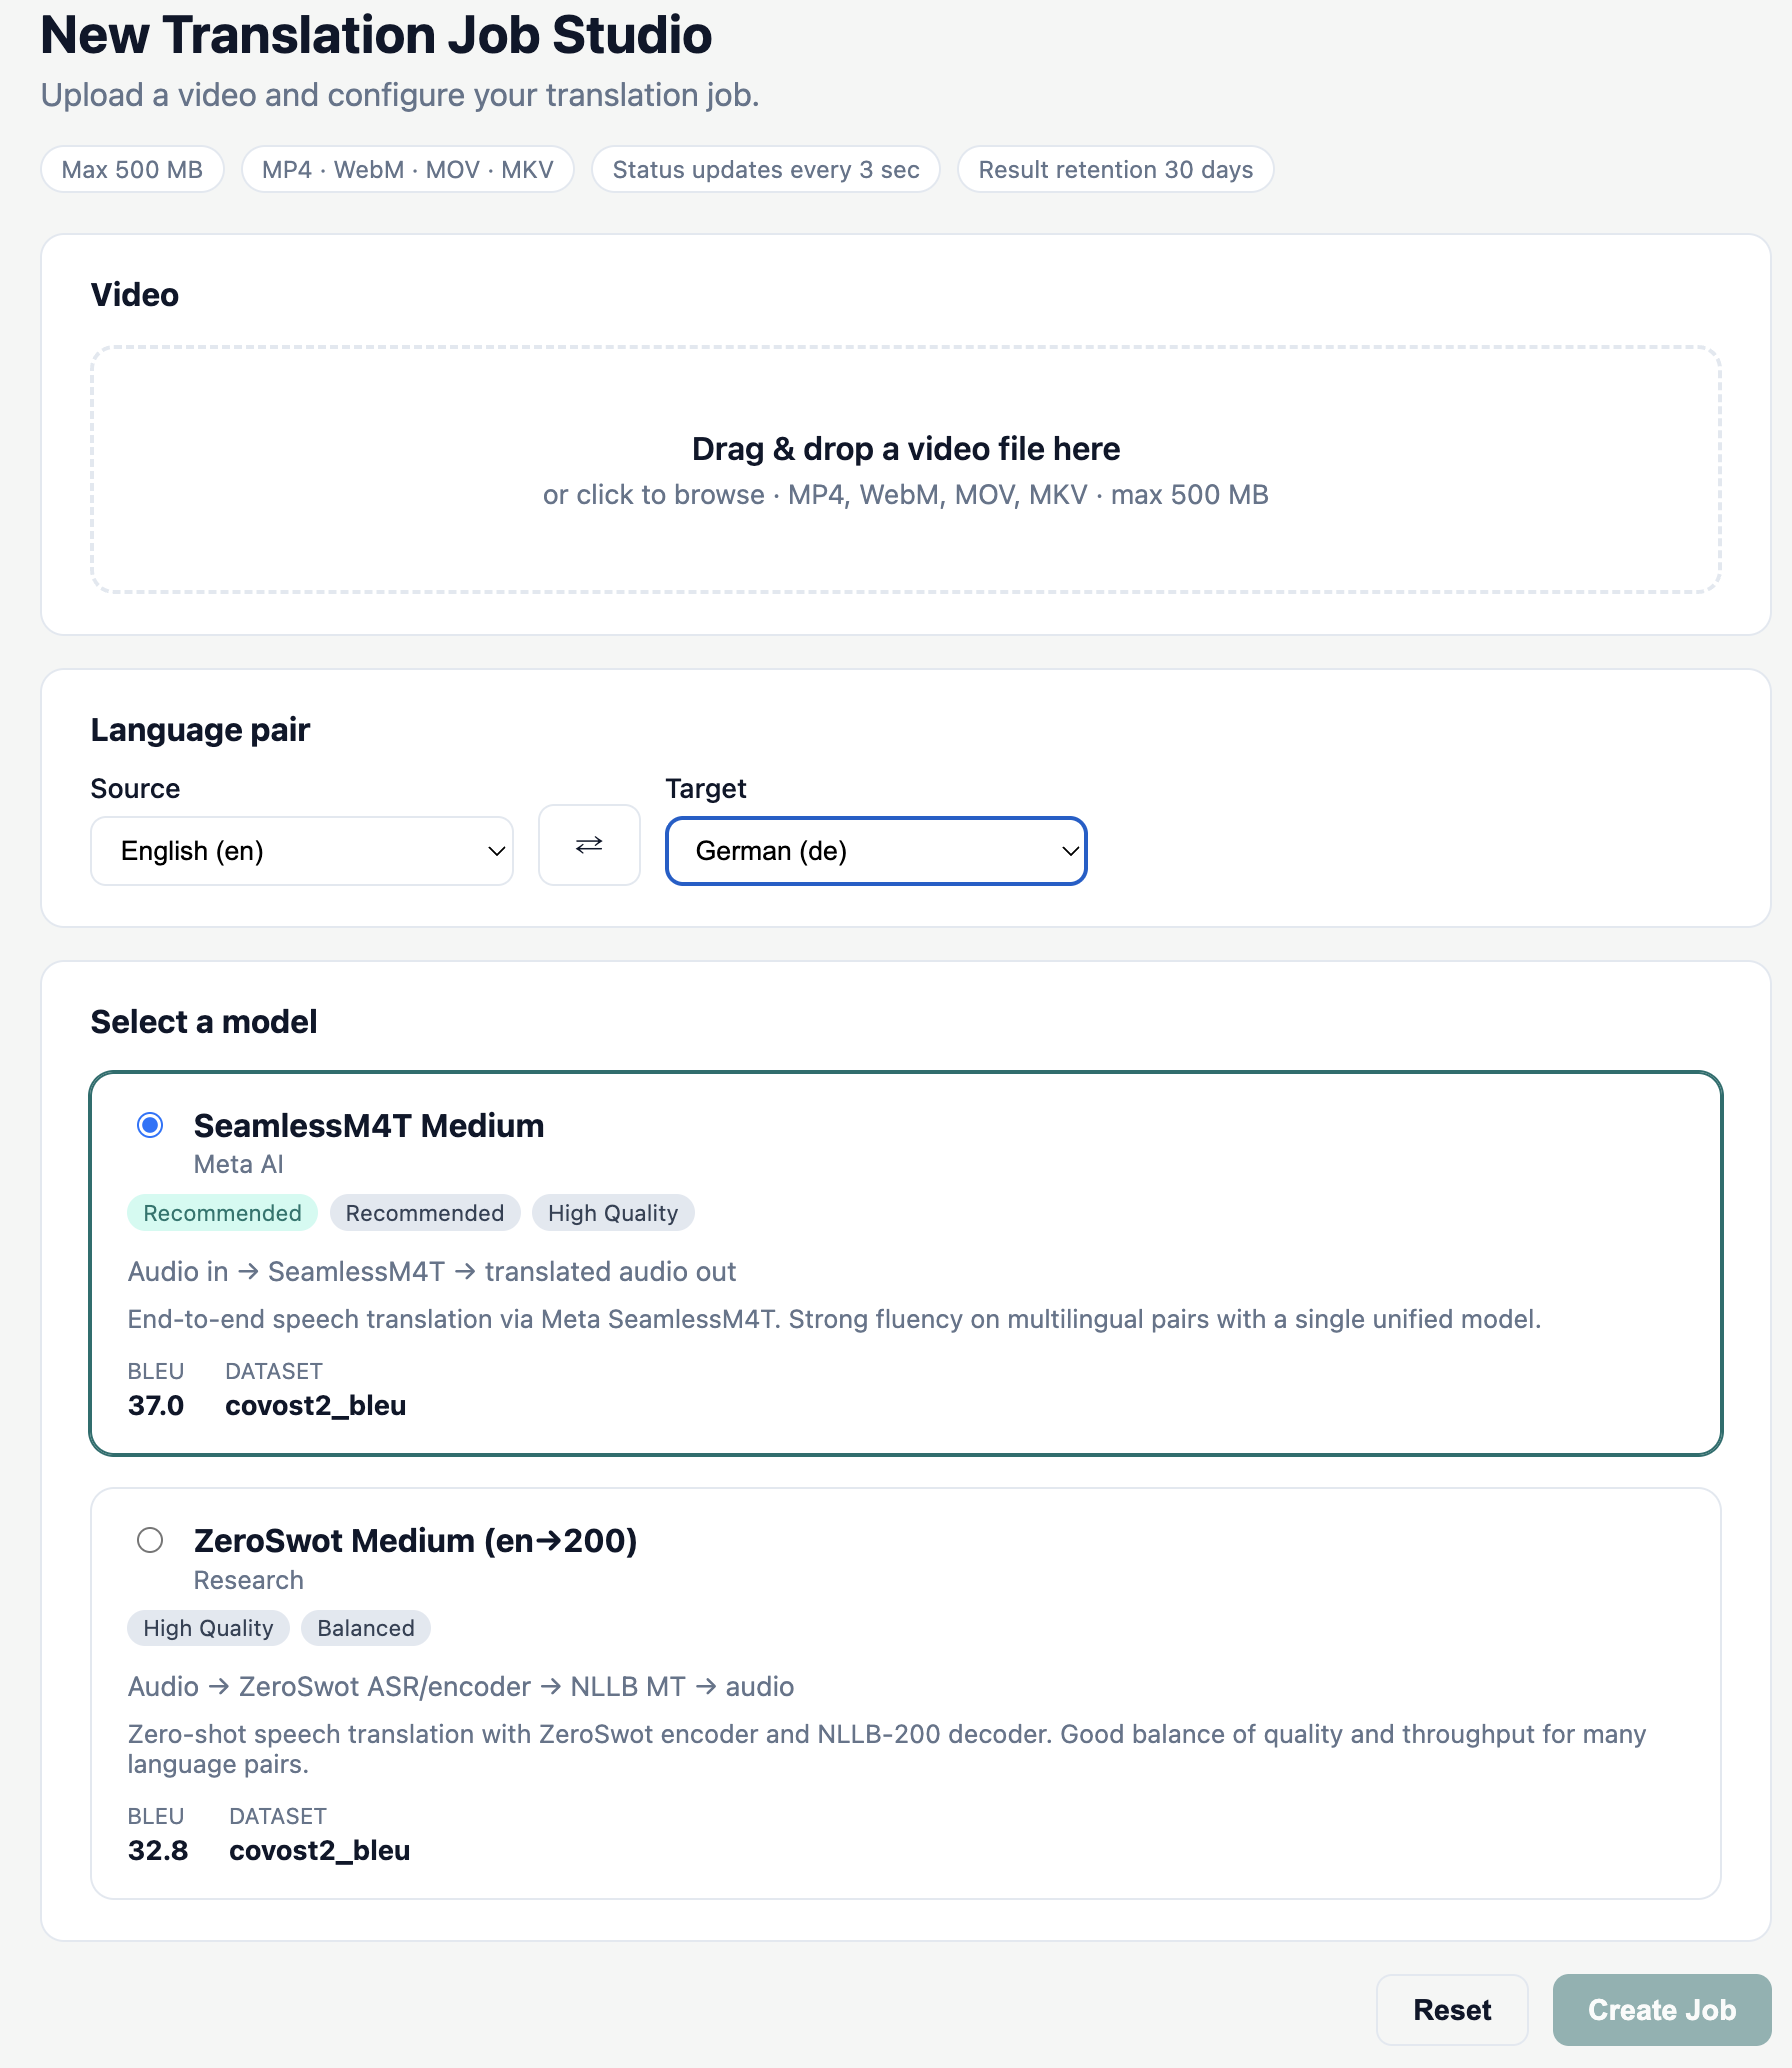
\includegraphics[width=0.75\textwidth]{images/frontend_interface_create_job.png}
\caption{
\label{fig:frontend-create-job}
     Интерфейс создания задачи перевода видео.}
\end{center}
\end{figure}

Основной внешний компонент, с которым взаимодействует фронтенд, --- сервис бэкенда. При выборе параметров перевода фронтенд запрашивает у сервиса доступные языки, модели для выбранной языковой пары, значения метрик качества и рекомендуемый вариант. Полученные данные используются только для отображения пользовательского состояния: фронтенд не принимает решений о доступности моделей самостоятельно, а опирается на сведения, возвращаемые серверной частью.

В сценарии загрузки видео фронтенд получает от бэкенда параметры загрузки и передаёт файл в хранилище в соответствии с ними. После этого он создаёт задачу перевода, передавая бэкенду ссылку на загруженный файл, исходный и целевой языки, а также выбранную модель. В ответ возвращается идентификатор задачи, который становится основой дальнейшего взаимодействия с системой.

Поскольку обработка видео выполняется асинхронно, фронтенд не ожидает завершения задачи в рамках одного запроса. Он периодически запрашивает у бэкенда текущее состояние задачи, прогресс, сообщение об ошибке и ссылку на результат, если обработка завершена успешно. Таким образом, фронтенд не зависит от деталей работы обработчиков, очередей и моделей машинного обучения: для пользовательского интерфейса система представлена последовательностью операций выбора параметров, загрузки файла, создания задачи, наблюдения за прогрессом и получения результата.

Для реализации фронтенда выбран React. Этот фреймворк удобен для построения интерфейсов, состояние которых зависит от данных, получаемых от бэкенда: списка моделей, рекомендации, статуса задачи и прогресса обработки. Компонентная модель React позволяет разделить экран на независимые части: выбор языков, список моделей, форму загрузки файла и блок отображения состояния задачи.

Код фронтенда пишется на TypeScript. Статическая типизация полезна для работы с ответами бэкенда: структура модели, задачи, статуса и сообщения об ошибке фиксируется в типах, поэтому часть ошибок интеграции обнаруживается ещё на этапе разработки. Для приложения, которое активно обменивается данными с серверной частью, это снижает риск некорректной обработки ответа API.

Для сборки приложения фронтенда используется Vite. Он обеспечивает быстрый запуск локальной среды разработки и сборку статических файлов для развёртывания. В контексте данной платформы это удобно, поскольку пользовательский интерфейс можно разрабатывать и проверять отдельно от тяжёлой части обработки видео, подключаясь к бэкенду как к внешнему сервису.

\subsection{База данных}

База данных хранит структурированные данные платформы: модели перевода, языковые пары, метрики качества и задачи обработки видео. Сами видеофайлы в базе не размещаются; для них хранятся только ключи объектов в хранилище. Такой подход разделяет метаданные и большие бинарные файлы.

В текущей схеме выделяются четыре основные таблицы:
\begin{itemize}
  \item \textbf{model} --- сведения о подключённых моделях перевода: служебный идентификатор, отображаемое имя, очередь обработчика, активность и конфигурация;
  \item \textbf{model\_language} --- направленные языковые пары для конкретной модели, внутренние коды языков и метрики качества перевода;
  \item \textbf{video} --- пользовательские задачи перевода: исходный файл, выбранная модель, языки, статус, прогресс, ключи объектов и сообщение об ошибке;
  \item \textbf{language} --- справочник языков и признаков поддержки речевого или текстового ввода и вывода.
\end{itemize}

Для реализации базы данных выбрана PostgreSQL. Она поддерживает транзакции, индексы, ограничения уникальности и JSON-поля, что удобно для хранения конфигурации моделей и ключей промежуточных артефактов. Метрики качества хранятся в таблице \textbf{model\_language}, поскольку качество перевода зависит не только от модели, но и от конкретной языковой пары.

\begin{figure}[H]
  \begin{center}
     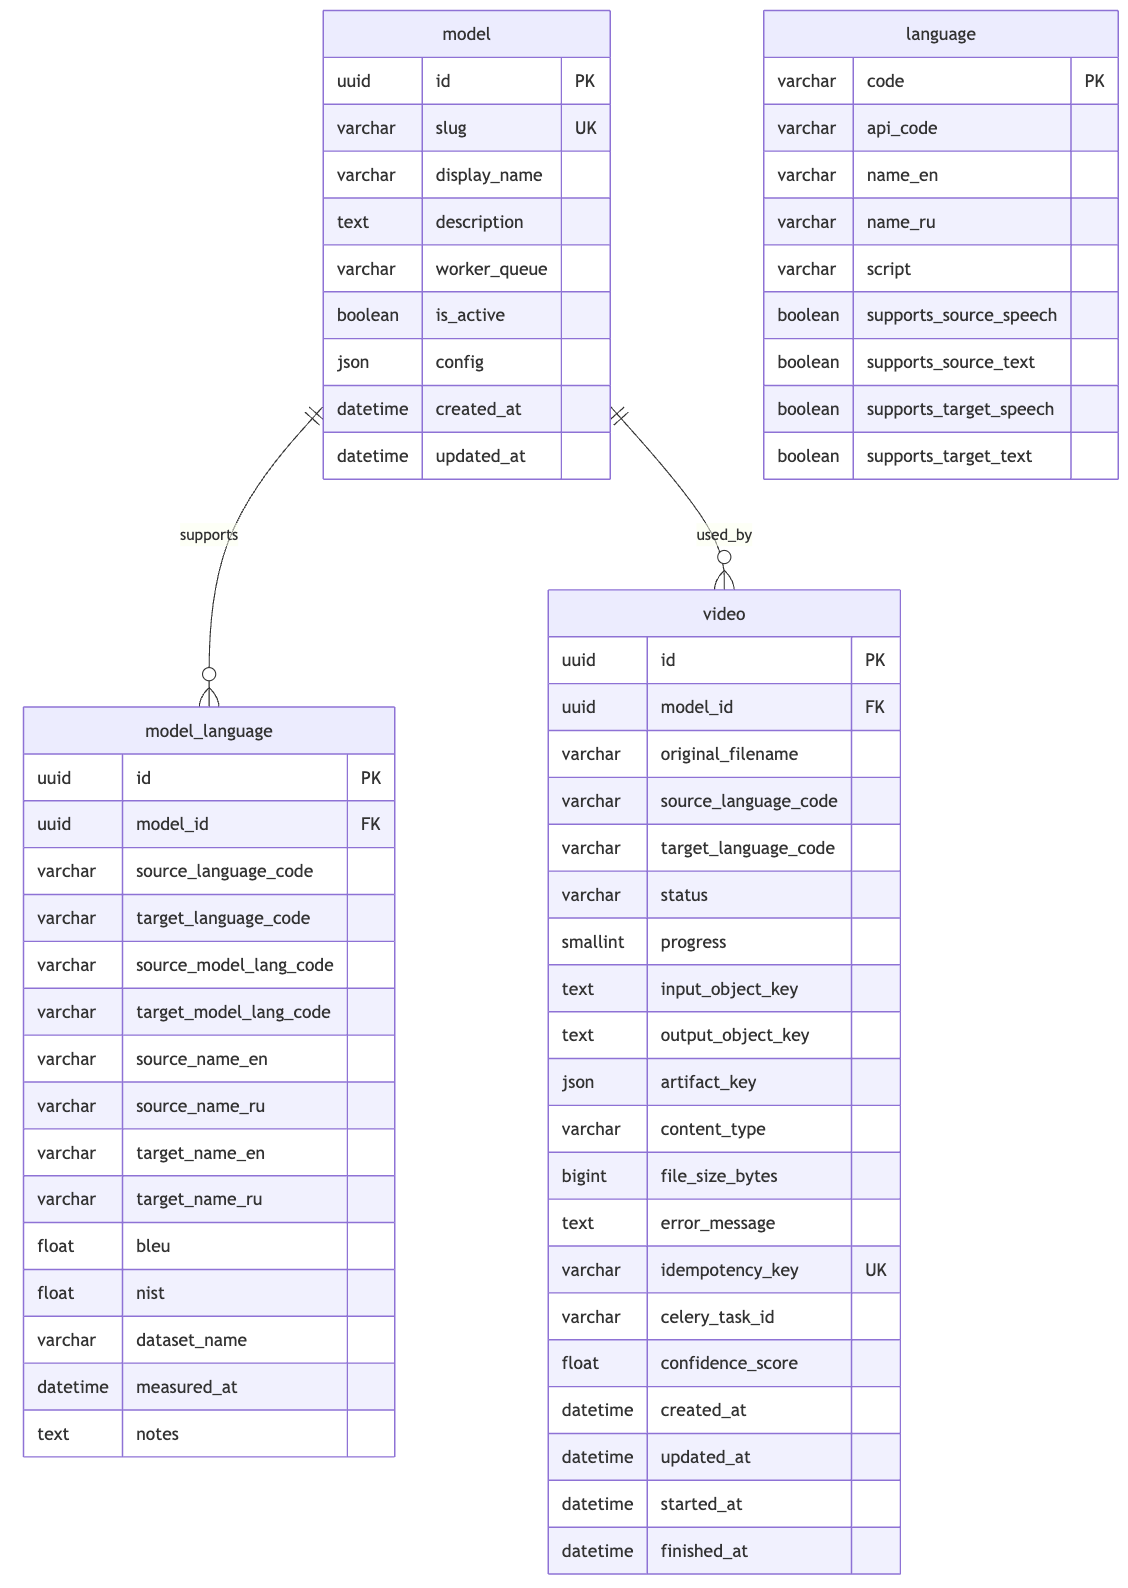
\includegraphics[height=0.60\textheight,keepaspectratio]{images/database.png}
  \caption{
  \label{fig:database-schema}
       Схема данных.}
  \end{center}
  \end{figure}

\subsection{Система администрирования}

Система администрирования используется для управления служебными данными платформы. Через неё администратор может добавлять и отключать модели, указывать поддерживаемые языковые пары, редактировать внутренние коды языков и обновлять значения метрик качества перевода.

Для реализации системы администрирования выбран Django Admin. Он автоматически строит интерфейс управления поверх моделей данных, поддерживает связи между таблицами и позволяет быстро получить рабочую административную панель без разработки отдельного приложения фронтенда. Это особенно удобно для ВКР, поскольку основное внимание можно уделить архитектуре платформы и обработке видео, а не написанию административного интерфейса с нуля.

\begin{figure}[H]
\begin{center}
   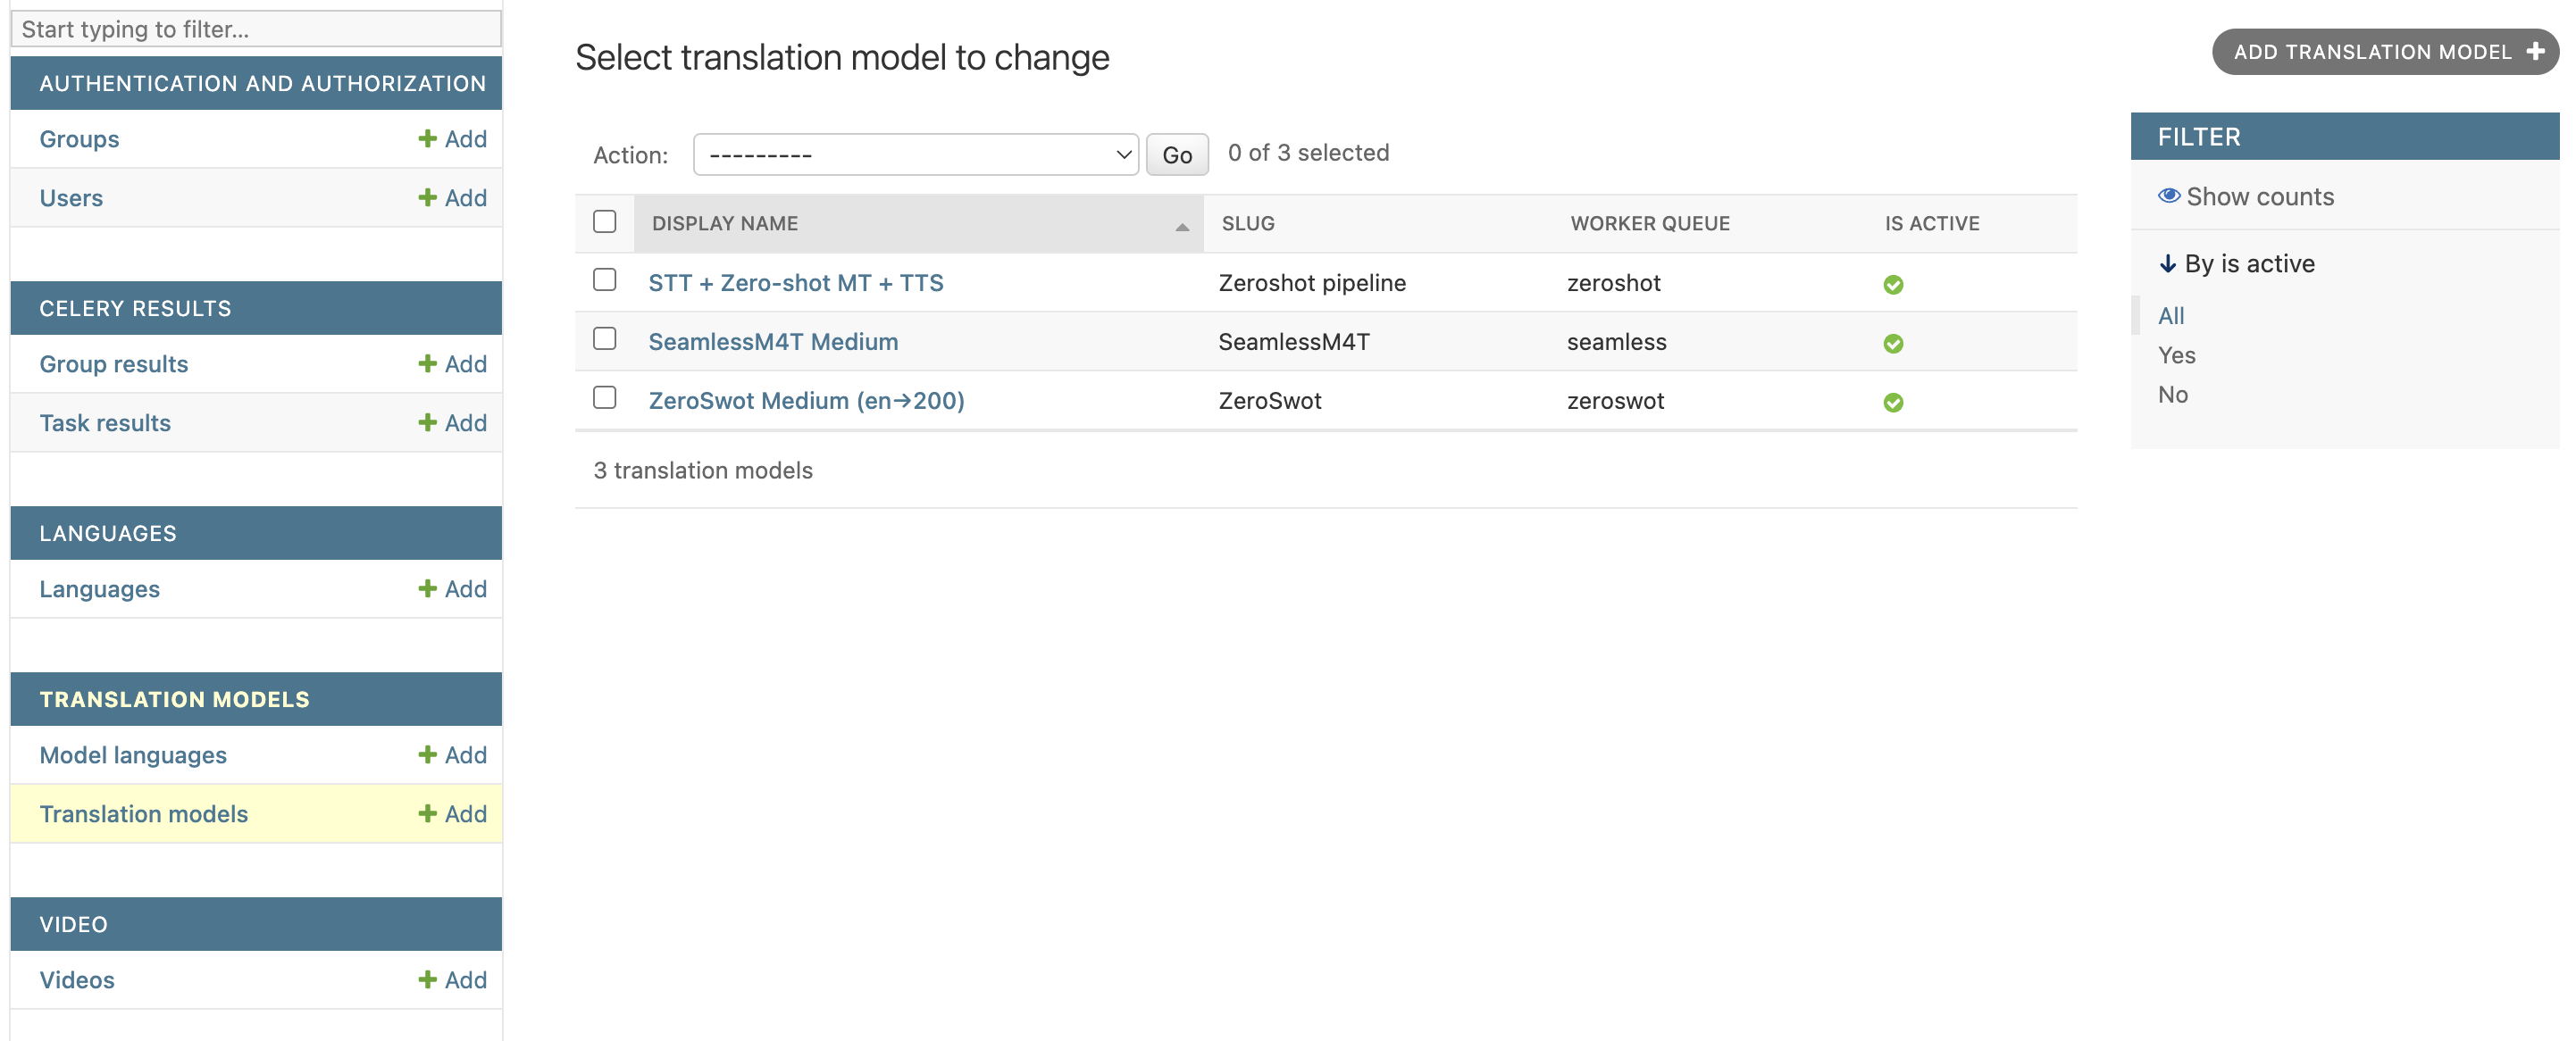
\includegraphics[width=0.95\textwidth]{images/admin_interface.png}
\caption{
\label{fig:admin-interface}
     Интерфейс системы администрирования.}
\end{center}
\end{figure}

\subsection{Бэкенд}

Бэкенд предоставляет программный интерфейс для фронтенда и управляет жизненным циклом задач перевода. Он отвечает за проверку входных параметров, получение списка доступных моделей, расчёт рекомендации, создание задачи, чтение статуса обработки и выдачу ссылки на готовый результат. С точки зрения пользовательского сценария бэкенд является центральным компонентом, который связывает интерфейс, базу данных, очередь задач и объектное хранилище.

При выборе языковой пары фронтенд обращается к бэкенду за списком моделей, поддерживающих это направление. Бэкенд получает сведения из базы данных, учитывает активность моделей и сохранённые метрики качества, после чего возвращает фронтенду список вариантов и рекомендуемую модель. Таким образом, логика доступности моделей и рекомендации сосредоточена на стороне бэкенда, а фронтенд только отображает полученный результат.

Отдельная часть ответственности бэкенда связана с загрузкой видео. Бэкенд не проксирует файл через себя и не принимает большой бинарный поток как основной сценарий работы. Вместо этого он создаёт подписанную ссылку для объектного хранилища, по которой фронтенд загружает видео напрямую. После завершения загрузки фронтенд передаёт бэкенду ключ загруженного объекта, а бэкенд создаёт запись о задаче в базе данных и передаёт сообщение в очередь.

Такой подход снижает нагрузку на бэкенд и уменьшает риск исчерпания памяти при одновременной загрузке нескольких больших видеофайлов. Бэкенд остаётся сервисом управления метаданными и задачами, а хранение больших файлов выносится в специализированное хранилище. Аналогичный принцип используется при получении результата: бэкенд проверяет состояние задачи и выдаёт ссылку на готовый файл, не передавая сам файл через процесс приложения.

Бэкенд не запускает модели машинного обучения самостоятельно. Это принципиальное решение: вывод модели может требовать GPU и занимать длительное время, тогда как HTTP-запросы должны завершаться быстро. Поэтому бэкенд создаёт задачу и передаёт её обработчику через очередь.

Для реализации бэкенда выбран Django REST Framework. Он позволяет описывать REST API поверх моделей Django, использовать валидацию входных данных и работать с PostgreSQL через Django ORM. Дополнительное преимущество состоит в том, что бэкенд и система администрирования используют одну модель данных, поэтому изменения в структуре сущностей отражаются согласованно.

Инфраструктура Django в бэкенде используется не только как слой маршрутов, но и как основа всей серверной части. Модели Django описывают основные сущности платформы: модель перевода, языковую пару, задачу обработки видео и справочник языков. На их основе формируются миграции базы данных, административный интерфейс и сериализаторы REST API. Это позволяет не дублировать структуру данных в разных частях приложения.

Маршрутизация запросов строится через представления Django REST Framework. Для каждого пользовательского сценария выделяется отдельная группа операций: получение языков и моделей, создание ссылки для загрузки видео, создание задачи, чтение состояния задачи и получение ссылки на результат. Сериализаторы используются для проверки входных данных и формирования ответов фронтенду, поэтому бэкенд возвращает данные в предсказуемом формате.

Для документирования программного интерфейса используется Swagger-интерфейс, представленный на рис.~\ref{fig:swagger}. Он позволяет просматривать доступные endpoints, параметры запросов и формат ответов. Такая документация полезна при разработке фронтенда, поскольку позволяет проверять контракт между интерфейсом пользователя и бэкендом без обращения к исходному коду серверной части.

\begin{figure}[H]
\begin{center}
   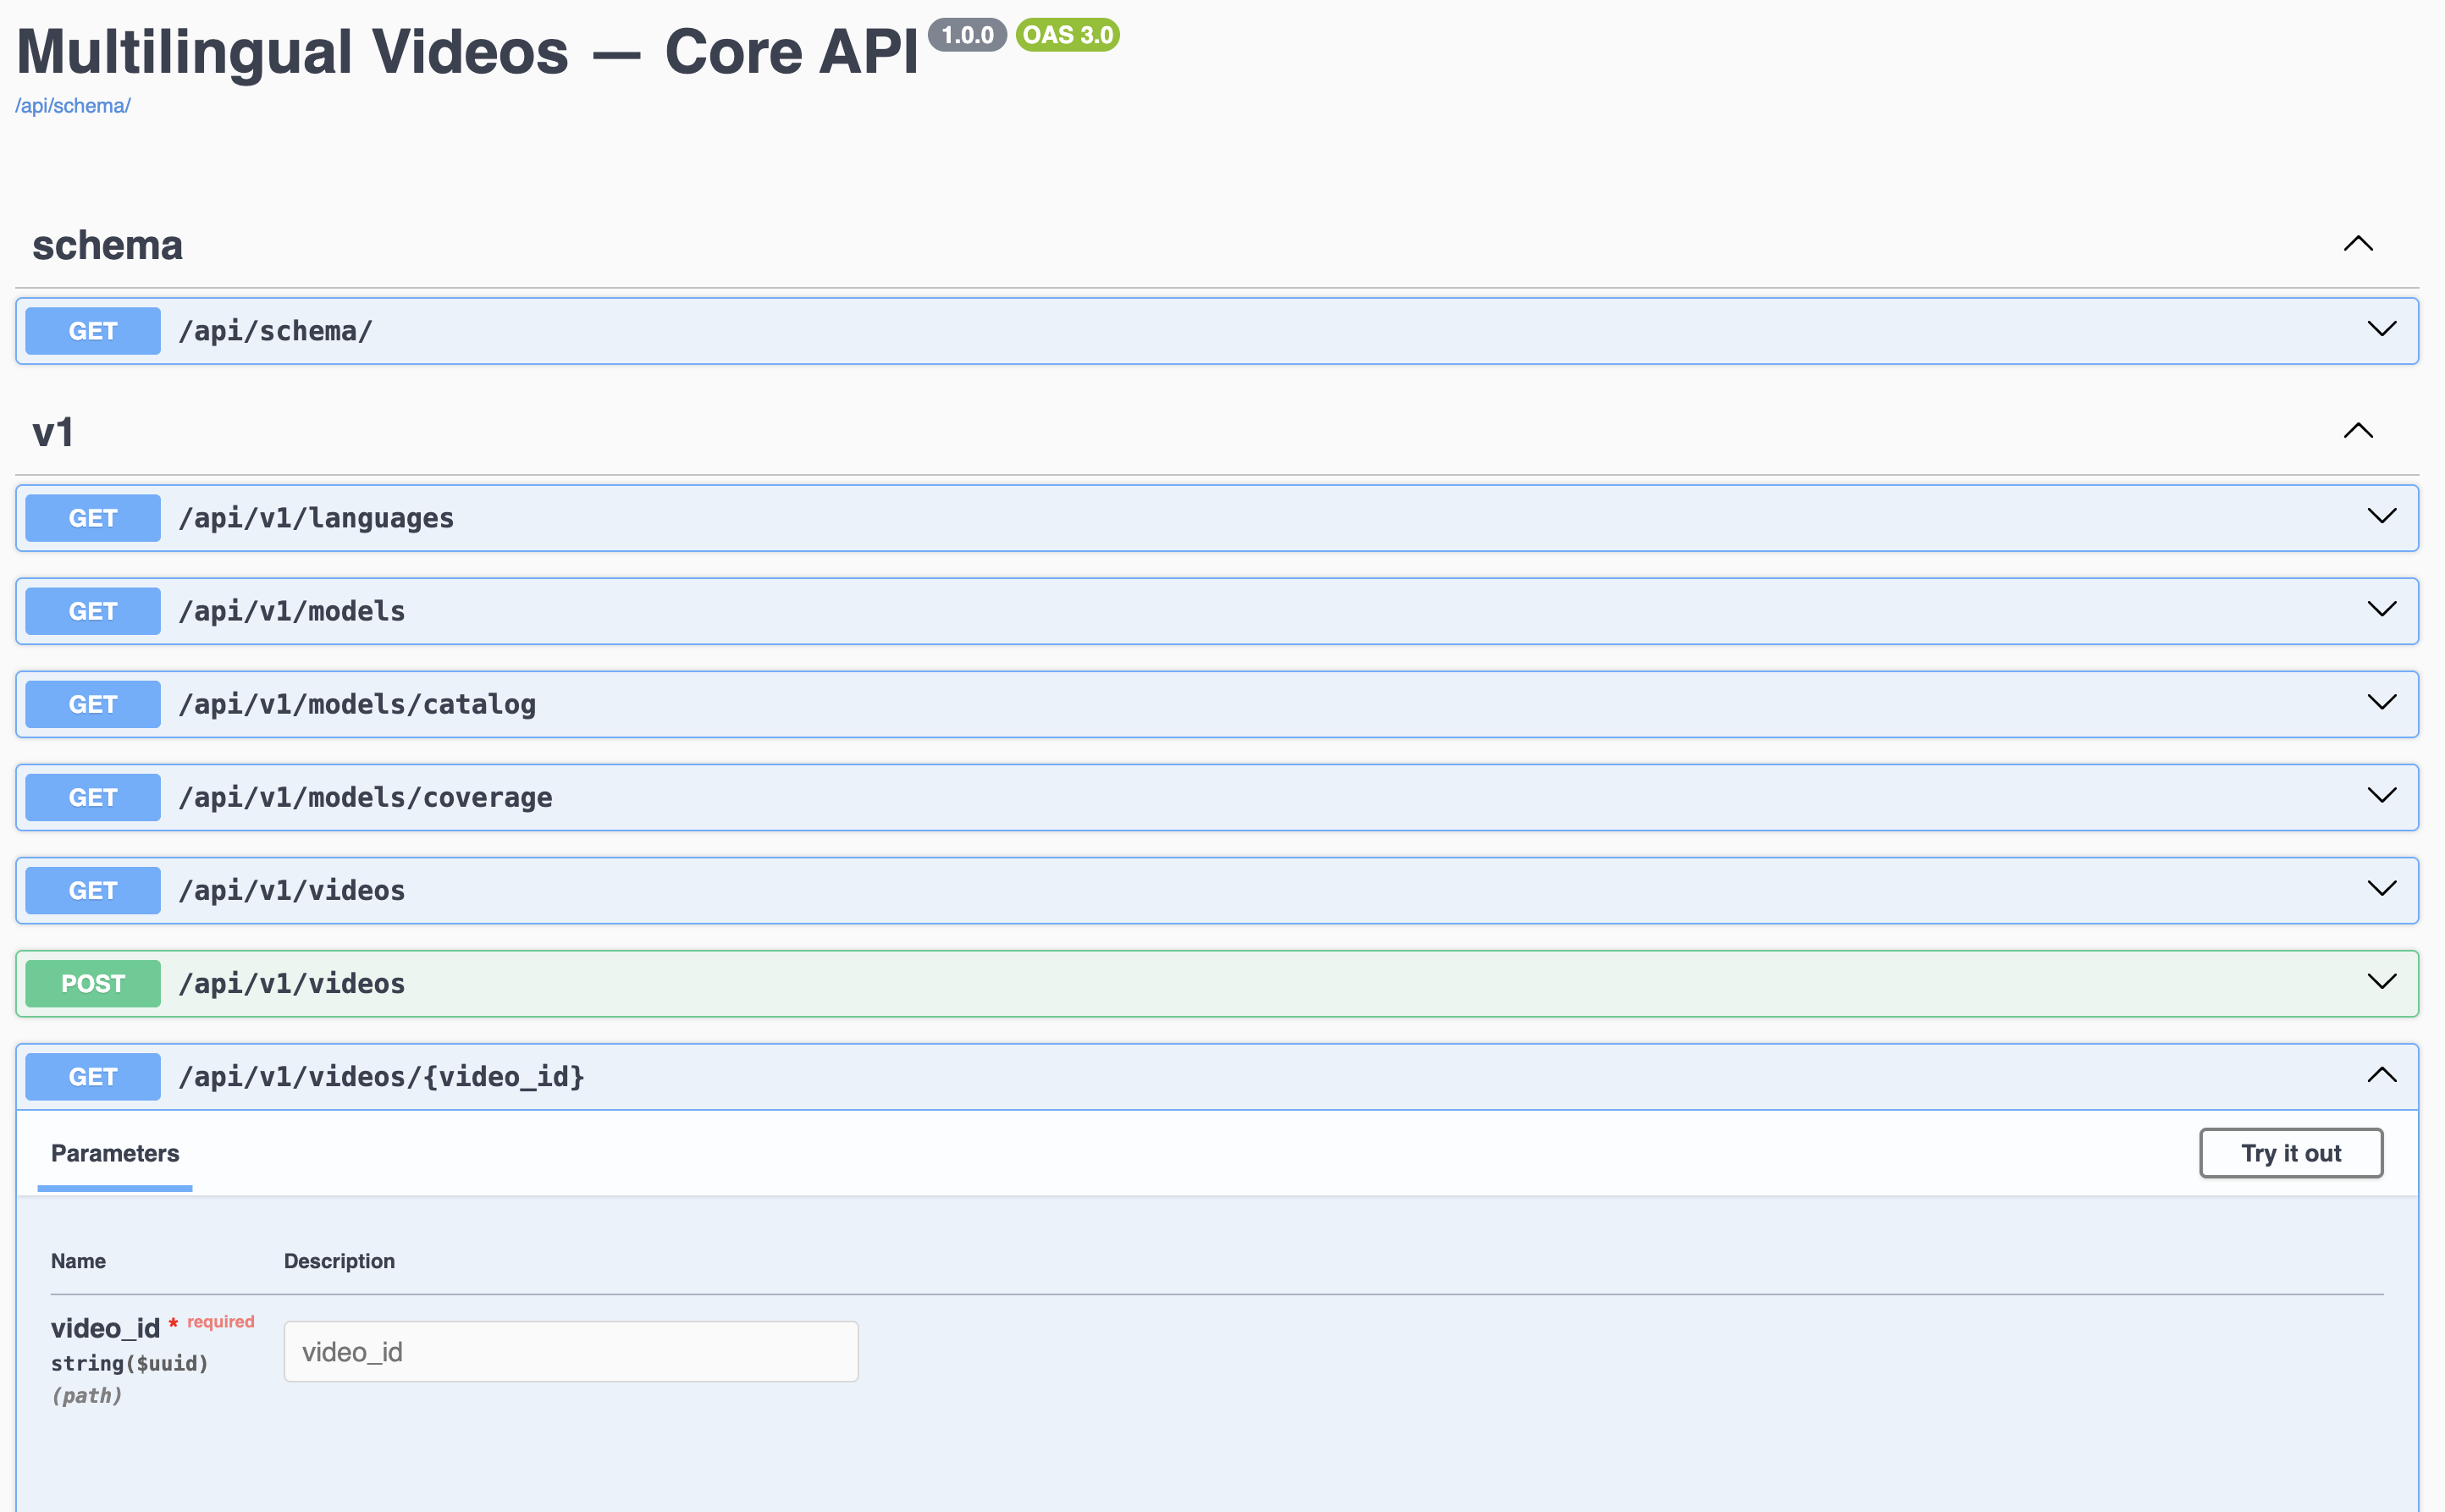
\includegraphics[width=0.95\textwidth]{images/swagger.png}
\caption{
\label{fig:swagger}
     Swagger-интерфейс бэкенда.}
\end{center}
\end{figure}

Настройки Django также используются для подключения внешних компонентов: базы данных PostgreSQL, объектного хранилища, очереди задач и параметров безопасности. Такой подход удобен для развёртывания, поскольку конфигурация может передаваться через переменные окружения и отличаться для локальной среды, тестового стенда и будущего серверного окружения. При этом код приложения остаётся одинаковым, а меняются только настройки подключения.

\subsection{Обработчик}

Обработчик выполняет ресурсоёмкую часть системы и изолирует бэкенд от работы с моделями машинного обучения и обработки медиафайлов. Он получает задачу из очереди, скачивает исходное видео из объектного хранилища, извлекает и нормализует аудио, разбивает его на фрагменты длительностью 5 секунд, запускает выбранный сценарий перевода, склеивает аудиофрагменты и собирает итоговое видео.

Важным требованием к обработчику является модульность. Общая логика обработки видео не должна зависеть от конкретной модели перевода, поскольку SeamlessM4T, ZeroSwot и собственная zero-shot схема имеют разные зависимости, форматы входных данных и требования к ресурсам. Поэтому обработчик строится вокруг общего интерфейса переводческого компонента: он передаёт в него нормализованный аудиофрагмент, исходный и целевой языки, а на выходе получает переведённый аудиофрагмент или данные, необходимые для его формирования.

Такой подход реализует зависимость от абстракций, а не от конкретных реализаций. Код, отвечающий за загрузку файлов, разбиение на фрагменты, обновление статуса задачи и сборку итогового видео, остаётся общим для всех моделей. При добавлении нового переводчика необходимо реализовать только адаптер, соответствующий общему интерфейсу, и зарегистрировать поддерживаемые языковые пары в базе данных.

Для запуска обработчиков используется Celery. Этот фреймворк предоставляет модель фоновых задач, повторные попытки выполнения и маршрутизацию по очередям. Для разных моделей могут использоваться разные очереди и разные экземпляры обработчика: это позволяет устанавливать отдельные зависимости, выделять разные вычислительные ресурсы и масштабировать только тот сценарий перевода, который является наиболее нагруженным.

\subsubsection{Сценарий Zeroshot}

Сценарий Zeroshot является каскадным вариантом обработки: исходный аудиофрагмент последовательно проходит через модель распознавания речи, модель машинного перевода и компонент синтеза речи. Сначала аудио преобразуется в текстовую расшифровку на исходном языке, затем полученный текст переводится собственной zero-shot моделью машинного перевода, после чего текст на целевом языке преобразуется в аудиофрагмент. Такой сценарий сохраняет явную границу между распознаванием речи, переводом и синтезом речи.

Преимущество такого сценария состоит в высокой наблюдаемости промежуточных результатов. После распознавания можно сохранить исходную расшифровку, после перевода --- текст на целевом языке, а после синтеза --- отдельный аудиофрагмент. Это упрощает отладку и позволяет определить, на каком этапе возникла ошибка: в распознавании речи, переводе или синтезе.

Сценарий Zeroshot также важен с точки зрения связи с исследовательской частью работы. Он позволяет подключить собственную модель машинного перевода как один из вариантов в платформе и сравнивать её с готовыми системами в одинаковом пользовательском контуре.

В данном сценарии для распознавания речи используется библиотека faster-whisper версии 1.0 и выше с моделью \foreignlanguage{english}{Whisper} \cite{Whisper}, поскольку она предоставляет готовый интерфейс для преобразования аудио в текст, поддерживает указание языка исходной речи и может эффективно выполняться на графическом ускорителе. Собственная zero-shot модель машинного перевода построена на архитектуре Transformer на базе TensorFlow версии 2.16 и выше и загружается в формате набора контрольных точек, так как обучение выполняется отдельно от платформы, а обработчик должен только применять готовые веса. Для синтеза речи используется edge-tts версии 6.1 и выше: эта библиотека предоставляет нейросетевые голоса для целевых языков и не требует отдельного графического ускорителя. При необходимости faster-whisper, TensorFlow-модель или edge-tts могут быть заменены другими реализациями, если они удовлетворяют тем же входным и выходным требованиям.

\subsubsection{Сценарий ZeroSwot}

Сценарий ZeroSwot предназначен для zero-shot перевода речи~\cite{ZeroSwot}. Он использует речевой энкодер, связанный с многоязычной моделью машинного перевода, поэтому входом для модели является аудиофрагмент, а не заранее подготовленный текст. В качестве переводческого декодера используется NLLB-200, поскольку эта модель поддерживает большое число языков и подходит для исследования многоязычного перевода.

В отличие от сценария Zeroshot, здесь часть промежуточных текстовых представлений может быть скрыта внутри модели. Это потенциально снижает число явно выделенных этапов, но усложняет диагностику ошибок: при неудовлетворительном результате труднее определить, была ли проблема связана с распознаванием, переводом или внутренним представлением речи.

Для платформы ZeroSwot рассматривается как отдельная реализация общего интерфейса переводчика. Бэкенд и остальная логика обработчика не зависят от того, как именно ZeroSwot строит перевод внутри модели. Обработчик передаёт входной аудиофрагмент и параметры языков, а результат сохраняется в том же формате артефактов, что и для других сценариев.

Для подключения ZeroSwot используется экосистема Hugging Face: библиотека Transformers версии 4.44 и выше позволяет загружать модель и токенизатор через единый интерфейс, PyTorch версии 2.4 и выше используется как основная среда выполнения нейросетевых вычислений, а Torchaudio версии 2.4 и выше применяется для приведения аудио к требуемой частоте дискретизации и формату. Дополнительно используется SentencePiece версии 0.2 и выше для работы с токенизацией. Такой выбор упрощает работу с готовыми весами модели и позволяет фиксировать конкретную версию модели, что важно для воспроизводимости экспериментов.

\subsubsection{Сценарий SeamlessM4T}

Сценарий SeamlessM4T использует готовую мультимодальную модель, поддерживающую несколько режимов перевода: speech-to-text, speech-to-speech, text-to-text и text-to-speech~\cite{SeamlessM4T}. Для платформы эта модель важна как сильная базовая реализация, поскольку она объединяет несколько направлений обработки речи и текста в одной системе.

В данном сценарии обработчик передаёт в модель предварительно подготовленный аудиофрагмент и параметры языковой пары, после чего получает результат перевода в одном из поддерживаемых моделью режимов. Это позволяет рассматривать SeamlessM4T как самостоятельный переводческий компонент, который скрывает значительную часть внутренней обработки речи и текста за единым интерфейсом.

Такое подключение удобно для платформы, поскольку общий порядок работы обработчика не меняется: загрузка исходного видео, разбиение на фрагменты, сохранение промежуточных данных и сборка итогового файла выполняются теми же средствами, что и для других сценариев. Отличается только адаптер модели, отвечающий за подготовку входных данных, вызов SeamlessM4T и приведение результата к общему формату артефактов задачи.

Для подключения SeamlessM4T используется библиотека Transformers версии 4.44 и выше, поскольку она предоставляет готовые классы процессора и модели SeamlessM4T, а также единый механизм загрузки весов из локального каталога или репозитория Hugging Face. Вычисления выполняются с помощью PyTorch версии 2.4 и выше, а предварительная обработка аудио и изменение частоты дискретизации выполняются средствами Torchaudio версии 2.4 и выше. Также используются SentencePiece версии 0.2 и выше для токенизации, Accelerate версии 0.34 и выше для настройки выполнения модели и Safetensors версии 0.4 и выше для работы с безопасным форматом хранения весов. Такой набор инструментов позволяет использовать готовую модель без самостоятельной реализации её архитектуры и сохраняет единый подход к работе с нейросетевыми моделями в обработчике.

\subsection{Инфраструктура}

Инфраструктурный слой обеспечивает работу платформы как распределённой системы. Его задача состоит не только в запуске отдельных сервисов, но и в организации надёжного обмена сообщениями, хранения файлов, развёртывания контейнеров и автоматизации поставки новых версий приложения.

\subsubsection{Очередь}

Для передачи длительных задач от бэкенда к обработчикам используется очередь сообщений. В качестве брокера выбран RabbitMQ: это система обмена сообщениями, которая принимает задачу от одного компонента и доставляет её другому компоненту, не требуя их одновременного выполнения в одном процессе. Для разрабатываемой платформы это особенно важно, поскольку перевод видео может занимать значительное время и не должен блокировать обработку HTTP-запросов.

RabbitMQ удобен для данной системы тем, что позволяет разделять задачи по очередям. Например, задачи для SeamlessM4T, ZeroSwot и собственной zero-shot схемы могут направляться в разные очереди и обрабатываться разными группами обработчиков. Это упрощает масштабирование и позволяет выделять ресурсы под конкретный тип модели.

Для наблюдения за состоянием фоновых задач используется Flower. Это web-интерфейс для Celery, через который можно просматривать активные и завершённые задачи, ошибки, повторные попытки и состояние обработчиков. Для платформы Flower полезен как инструмент эксплуатации и отладки: пользовательский интерфейс получает статус задачи из базы данных, а администратор или разработчик может использовать Flower для анализа работы очередей и поиска причин сбоев.

\subsubsection{S3-хранилище}

S3-совместимое объектное хранилище используется для исходных видео, промежуточных артефактов и итоговых файлов. База данных хранит только метаданные задачи, статусы и ключи объектов, а сами файлы выносятся во внешнее хранилище. Такое разделение уменьшает нагрузку на базу данных и упрощает работу с крупными видеофайлами.

От S3-хранилища требуется несколько свойств. Оно должно поддерживать хранение больших бинарных объектов, устойчивое долговременное хранение файлов, разграничение доступа и возможность выдачи временных подписанных ссылок. Подписанные ссылки позволяют фронтенду загружать исходное видео и скачивать результат напрямую из хранилища, не передавая большие файлы через бэкенд. Кроме того, единый объектный слой удобен для сохранения промежуточных данных: аудиофрагментов, расшифровок, переводов и результатов обработки отдельных фрагментов.

Для работы с S3 API используется библиотека boto3. Она предоставляет стандартный Python-интерфейс для загрузки и скачивания объектов, формирования подписанных ссылок и управления ключами файлов. Использование boto3 позволяет не привязывать код платформы к конкретной реализации объектного хранилища, если она совместима с S3 API.

\subsubsection{Docker Swarm}

Для развёртывания набора сервисов используется Docker Swarm. Это встроенный в Docker механизм оркестрации контейнеров, который позволяет запускать приложение как набор сервисов на одном или нескольких серверах. В отличие от локального запуска через Docker Compose, Docker Swarm предназначен для более длительной эксплуатации и поддерживает управление репликами, сетями, секретами и обновлениями сервисов.

В реализованной платформе Docker Swarm используется для запуска фронтенда, бэкенда, очереди, базы данных, системы мониторинга задач и обработчиков как отдельных сервисов. Бэкенд и фронтенд масштабируются как stateless-сервисы, очередь и база данных разворачиваются как инфраструктурные сервисы, а обработчики размещаются на узлах с необходимыми вычислительными ресурсами. Кроме того, Docker Swarm обеспечивает rolling update, то есть постепенную замену старой версии сервиса новой без полной остановки платформы.

\subsubsection{CI/CD}

Для автоматизации проверки и поставки новых версий используется GitHub Actions. На уровне continuous integration сценарии GitHub Actions выполняют базовые проверки: установку зависимостей, статический анализ кода, запуск тестов и проверку сборки контейнеров. Это снижает риск попадания ошибок в основную ветку разработки.

На уровне continuous delivery тот же механизм используется для подготовки релизов. После создания тега или слияния изменений в основную ветку GitHub Actions собирает Docker-образы, публикует их в реестр контейнеров и запускает сценарий развёртывания на сервере. Для платформы перевода видео это важно, поскольку релиз затрагивает несколько компонентов одновременно: фронтенд, бэкенд, обработчики и инфраструктурные настройки.

\newpage
\section{Тестирование}

Тестирование платформы проводилось для проверки корректности основных пользовательских сценариев, устойчивости серверной части и практической применимости подключённых моделей перевода. Отдельно проверялись качество результата для разных подходов, автоматические тесты бэкенда и ручная обработка видеороликов разной длительности.

\subsection{Сравнение моделей}

Сравнение результатов перевода выполнялось для трёх подключённых подходов: собственной каскадной схемы Zeroshot, модели ZeroSwot и модели SeamlessM4T. Все модели запускались через общий интерфейс обработчика, поэтому входные данные, разбиение видео на фрагменты, сохранение промежуточных артефактов и сборка итогового видео выполнялись одинаковым образом. Это позволяет сравнивать не только сами модели, но и их поведение в едином прикладном контуре.

Исследование качества перевода проводилось на данных OPUS для направления $\textbf{De}\!\rightarrow\!\textbf{Uk}$. В качестве автоматических метрик использовались BLEU и NIST; полученные значения приведены в таблице.

\begin{center}
\begin{longtable}{|p{6cm}|p{3cm}|p{3cm}|}
\caption{Результаты сравнения моделей перевода на данных OPUS.}\\
\hline
Модель & BLEU & NIST\\
\hline
ZeroShot (baseline) & 0{,}1110 & 0{,}1080\\
\hline
ZeroShot (лекс. сходство) & 0{,}1320 & 0{,}1280\\
\hline
ZeroSwot + NLLB-600M & 0{,}0403 & 0{,}0477\\
\hline
ZeroSwot Large & 0{,}1277 & 0{,}1103\\
\hline
\textbf{SeamlessM4T Medium} & \textbf{0{,}1590} & \textbf{0{,}1483}\\
\hline
\end{longtable}
\end{center}

По результатам измерений наилучшие значения обеих метрик были получены для SeamlessM4T Medium. Это позволяет использовать данную модель как рекомендуемый вариант для рассматриваемого направления перевода, сохраняя при этом возможность выбора других подходов через интерфейс платформы.

\subsection{Покрытие тестами}

Для бэкенда были реализованы unit-тесты, покрывающие основные операции работы с моделями, языковыми парами и задачами обработки видео. Покрытие бэкенда unit-тестами составило 54\%. Это значение отражает проверку ключевой бизнес-логики: выбора доступных моделей для языковой пары, создания задач, переходов между статусами и формирования ссылок для работы с объектным хранилищем.

Помимо unit-тестов были написаны интеграционные тесты. Они проверяют взаимодействие нескольких компонентов системы: бэкенда, базы данных, очереди задач и объектного хранилища. Такие проверки важны, поскольку основные пользовательские сценарии платформы связаны не с отдельной функцией, а с последовательностью действий: выбором модели, загрузкой видео, созданием задачи, запуском обработки и получением результата.

\subsection{Ручное тестирование}

Ручное тестирование проводилось на видеороликах длительностью 10, 30 и 60 минут. Проверялись основные пользовательские сценарии: выбор языковой пары и модели, загрузка исходного видео, создание задачи обработки, отображение прогресса, завершение задачи и получение готового файла. Также проверялась работа административного интерфейса для просмотра и изменения сведений о моделях и языковых парах.

Тестирование выполнялось на инфраструктуре, включающей два CPU-сервера и один GPU-сервер. CPU-серверы использовались для размещения сервисов, не требующих графического ускорителя, а GPU-сервер --- для запуска обработчиков с моделями машинного обучения.

\begin{table}[H]
\begin{center}
\caption{Ресурсы, использованные при ручном тестировании.}
\begin{tabular}{|p{3.5cm}|p{9.5cm}|}
\hline
Тип сервера & Характеристики\\
\hline
CPU-серверы & 2 сервера по 4 ядра CPU 2,8 ГГц, 4 ГБ DDR4, 80 ГБ SSD NVMe\\
\hline
GPU-сервер & NVIDIA 1xA4000 16 ГБ, 16 vCPU, 64 ГБ RAM, 256 ГБ дискового пространства\\
\hline
\end{tabular}
\end{center}
\end{table}

По результатам ручного тестирования было измерено время обработки видеороликов разной длительности для каждого из трёх подходов. Полученные значения представлены в таблице.

\begin{center}
\begin{longtable}{|p{4cm}|p{3cm}|p{3cm}|p{3cm}|}
\caption{Время обработки видеороликов разной длительности.}\\
\hline
Длительность исходного видео & Zeroshot & ZeroSwot & SeamlessM4T\\
\hline
10 минут & 27 минут & 14 минут & 8 минут\\
\hline
30 минут & 54 минуты & 43 минуты & 35 минут\\
\hline
60 минут & 1 ч 49 минут & 1 ч 12 минут & 57 минут\\
\hline
\end{longtable}
\end{center}

Полученные результаты показывают, что время обработки зависит не только от длительности исходного видео, но и от выбранного подхода. Наименьшее время обработки для всех трёх длительностей показала модель \foreignlanguage{english}{SeamlessM4T}; это связано с использованием готовой мультимодальной модели и меньшим числом явно выделенных этапов обработки. Каскадный сценарий Zeroshot требует больше времени из-за последовательного выполнения распознавания речи, машинного перевода и синтеза речи.

\newpage
\section{Перспективы развития платформы}

\subsection{Генерация субтитров}

Одним из направлений развития платформы является генерация субтитров к видео. Пользователь может получать не только ролик с заменённой аудиодорожкой, но и файл субтитров на исходном или целевом языке. Такой формат полезен для образовательных материалов, лекций и рабочих встреч, где не всегда требуется полная переозвучка видео.

Поддержка субтитров расширяет набор пользовательских сценариев. Пользователь сможет выбрать формат результата: только переведённое видео, только субтитры или оба варианта одновременно. Дополнительно субтитры могут использоваться как промежуточный результат для проверки качества распознавания и перевода перед запуском синтеза речи.

\subsection{Редактор результата перед публикацией}

Вторым продуктовым направлением является встроенный редактор результата. После автоматической обработки пользователь сможет просмотреть распознанный текст, перевод и разбиение на временные фрагменты, внести правки и только после этого запустить финальную сборку видео. Такой сценарий особенно важен для материалов, где требуется не черновой перевод, а публикация для внешней аудитории.

Редактор может снижать стоимость ручной доработки результата. Вместо полного повторного перевода пользователь исправляет только проблемные фрагменты: неточности распознавания, неверные термины, слишком длинные фразы или неудачные формулировки. После сохранения изменений платформа повторно выполняет только необходимые этапы обработки, например синтез речи и сборку итогового видео.

\newpage
\specialsection{Выводы}

В рамках данной работы была разработана система перевода видеоконтента с использованием zero-shot translation.

Целью работы было создание платформы, позволяющей пользователю загружать видео, выбирать модель перевода, отслеживать ход обработки и получать готовый файл с переведённой аудиодорожкой. Для достижения этой цели была спроектирована и реализована модульная система, в которой бэкенд, фронтенд, система администрирования, база данных, очередь задач, объектное хранилище и обработчики разделены по зонам ответственности.

В работе были выполнены следующие задачи:
\begin{itemize}
  \item рассмотрены подходы к многоязычному и zero-shot переводу, а также каскадные и end-to-end подходы к переводу видеоконтента;
  \item спроектирована архитектура платформы с асинхронной обработкой задач, хранением файлов в S3-совместимом хранилище и отдельными обработчиками для разных моделей;
  \item реализованы пользовательский интерфейс, бэкенд, система администрирования, база данных и инфраструктурный контур;
  \item подключены три сценария обработки: Zeroshot, ZeroSwot и SeamlessM4T;
  \item проведено сравнение моделей на данных OPUS для направления $\textbf{De}\!\rightarrow\!\textbf{Uk}$ с использованием метрик BLEU и NIST;
  \item выполнено автоматическое и ручное тестирование платформы.
\end{itemize}

По результатам исследования качества перевода наилучшие значения BLEU и NIST среди рассмотренных моделей были получены для SeamlessM4T Medium. При этом архитектура платформы не ограничена одной моделью: новые переводчики могут подключаться через общий интерфейс обработчика и регистрироваться в системе администрирования вместе с поддерживаемыми языковыми парами и метриками качества.

Тестирование показало, что система поддерживает основные пользовательские сценарии: выбор модели, загрузку видео, создание задачи, отображение прогресса, получение результата и управление сведениями о моделях через административный интерфейс. Также были проведены замеры времени обработки роликов длительностью 10, 30 и 60 минут для всех трёх подходов.

\newpage
\specialsection{Заключение}

В данной работе была рассмотрена задача автоматического перевода видеоконтента с использованием zero-shot translation.

В качестве основы были использованы результаты предыдущих исследований zero-shot перевода, однако в данной работе задача была расширена до прикладного сценария обработки видео. Если в текстовом переводе основным результатом является последовательность предложений на целевом языке, то в переводе видеоконтента необходимо дополнительно извлечь аудио, распознать речь, выполнить перевод, синтезировать новую аудиодорожку и собрать итоговый видеофайл.

В ходе работы была реализована платформа, поддерживающая несколько подходов к переводу: собственную каскадную схему Zeroshot, ZeroSwot и SeamlessM4T. Для пользователя система предоставляет единый сценарий работы: загрузку исходного видео, выбор модели, запуск обработки, наблюдение за прогрессом и получение результата. Для администратора предусмотрено управление сведениями о моделях, языковых парах и метриках качества.

Экспериментальная часть показала, что для направления $\textbf{De}\!\rightarrow\!\textbf{Uk}$ на данных OPUS наилучшие значения BLEU и NIST среди рассмотренных вариантов демонстрирует SeamlessM4T Medium. Дополнительно было проведено тестирование производительности на роликах разной длительности, а также проверены основные пользовательские сценарии платформы.

Практическим результатом работы является модульная система, пригодная для дальнейшего расширения. В неё можно добавлять новые модели перевода, новые языковые пары и новые форматы результата. Перспективными продуктовыми направлениями развития являются генерация субтитров и редактор результата перед публикацией.

% Библиография в cpsconf стиле
% Аргумент {1} ниже включает переопределенный стиль с выравниванием слева
\begin{thebibliography}{11}
\bibitem{Google} Johnson~M., Schuster~M., Le~Q.~V. et~al. Google's multilingual neural machine translation system: enabling zero-shot translation // Transactions of the Association for Computational Linguistics. 2017. Vol.~5. P.~339--351.

\bibitem{Devrishev2023} Девришев~Н.~Э. Улучшение перевода zero-shot с использованием лексического сходства языков // Процессы управления и устойчивость. 2023. Т.~10. №~1. С.~250--258.

\bibitem{bleu} Papineni~K., Roukos~S., Ward~T., Zhu~W.-J. BLEU: a method for automatic evaluation of machine translation // Proceedings of the 40th Annual Meeting of the Association for Computational Linguistics. 2002. P.~311--318.

\bibitem{nist} Przybocki~M., Peterson~K., Bronsart~S., Sanders~G. The NIST 2008 metrics for machine translation challenge -- overview, methodology, metrics, and results // Machine Translation. 2009. Vol.~23. P.~71--103.

\bibitem{Attention} Vaswani~A., Shazeer~N., Parmar~N. et~al. Attention is all you need // Proceedings of the 31st International Conference on Neural Information Processing Systems. 2017. P.~6000--6010.

\bibitem{opus_1} Tiedemann~J. Parallel data, tools and interfaces in OPUS // Proceedings of the 8th International Conference on Language Resources and Evaluation. 2012.

\bibitem{opus_2} Lison~P., Tiedemann~J. OpenSubtitles2016: extracting large parallel corpora from movie and TV subtitles // Proceedings of the 10th International Conference on Language Resources and Evaluation. 2016.

\bibitem{Whisper} Radford~A., Kim~J.~W., Xu~T. et~al. Robust speech recognition via large-scale weak supervision // Proceedings of the 40th International Conference on Machine Learning. 2023. P.~28492--28518.

\bibitem{ZeroSwot} Tsiamas~I., G{\'a}llego~G.~I., Fonollosa~J.~A.~R., Costa-juss{\`a}~M.~R. Pushing the limits of zero-shot end-to-end speech translation // Findings of the Association for Computational Linguistics: ACL. 2024. P.~14245--14267.

\bibitem{SeamlessM4T} Barrault~L., Chung~Y.-A., Meglioli~M.~C. et~al. Joint speech and text machine translation for up to 100 languages // Nature. 2024. Vol.~631. P.~308--312.

\bibitem{XTTS} Casanova~E., Weber~J., Shulby~C.~D. et~al. XTTS: a massively multilingual zero-shot text-to-speech model // Proceedings of ICASSP. 2024.

\end{thebibliography}

\newpage

\specialsection{Приложение A. Реализация.}

Реализация системы перевода видеоконтента доступна в GitHub-репозитории по ссылке:

\url{https://github.com/RolfAdolf/multilingual-vids}

\end{document}
% TODO: добавить описание каждой модели в подходы
% TODO: добавить мониторинг